\documentclass[a4paper,12pt]{article}

\newcommand{\me}{Jonathan R.\ J.\ Yong}
\newcommand{\meshort}{J.R.J.Y.}
\newcommand{\eriks}{{\=E}riks Kup{\v{c}}e}
\newcommand{\tim}{Tim D. W. Claridge}

% Fonts {{{1
\usepackage{fontspec}
\usepackage{amsmath}
\usepackage{mathtools}
\usepackage[warnings-off={mathtools-colon,mathtools-overbracket}]{unicode-math}

% Main fonts used in the document
\setmainfont[
  Path={./fonts/},
  Extension=.otf,
  UprightFont={*-regular},
  BoldFont={*-semibold},
  ItalicFont={*-italic},
  BoldItalicFont={*-semibolditalic},
  Ligatures=TeX,
]{minion3}
\setmonofont[
  Path={./fonts/},
  Extension=.ttf,
  UprightFont={*-Regular},
  BoldFont={*-SemiBold},
  ItalicFont={*-Italic},
  BoldItalicFont={*-SemiBoldItalic},
  Scale=MatchLowercase
]{RobotoMono}
\setmathfont[
  Path={./fonts/},
  Scale=MatchLowercase,
  Ligatures=TeX,
]{MinionMath-Regular.otf}
\mathitalicsmode=1

% Other optical sizes for Minion
\newfontfamily{\fontcaption}{minion3caption}[
  Path={./fonts/},
  Extension=.otf,
  UprightFont={*-regular},
  BoldFont={*-semibold},
  ItalicFont={*-italic},
  BoldItalicFont={*-semibolditalic},
  Ligatures=TeX,
]
\newfontfamily{\fontsubhead}{minion3subhead}[
  Path={./fonts/},
  Extension=.otf,
  UprightFont={*-regular},
  BoldFont={*-bold},
  ItalicFont={*-italic},
  BoldItalicFont={*-bolditalic},
  Ligatures=TeX,
]

\usepackage{microtype}
% }}}1
% Packages and settings {{{1
\usepackage[font=small,labelfont=it,margin=15pt,skip=5pt]{caption}
\usepackage{fullpage,parskip,graphicx,float,braket,setspace,subcaption,booktabs}
\usepackage[svgnames]{xcolor}

% \usepackage{minted}
% \usepackage{tcolorbox}
% \tcbuselibrary{minted}
% \renewcommand{\MintedPygmentize}{./pygmentize_bruker.py}
% \usepackage{listings}
% \lstset{upquote=true}
% \newtcblisting{tcbminted}[1]{%
%     colframe=black,%
%     colback=white,%
%     width=0.95\textwidth,%
%     center,%
%     listing only,%
%     minted options={curlyquotes=false,fontsize=\small},%
%     minted language={#1},%
% }

\usepackage{chemformula}
\setchemformula{math-scripts=true}
\usepackage[style=chem-acs,subentry,articletitle,doi]{biblatex}
\addbibresource{hcosy.bib}
\graphicspath{{./figures/}}
\usepackage{xurl}   % must be after biblatex
\usepackage[
  mode=match,
  range-phrase={--},
  range-units=single,
  propagate-math-font=true,
  reset-math-version=false,
  reset-text-family=false,
  reset-text-series=false,
  text-family-to-math=true,
  text-series-to-math=true
]{siunitx}
\usepackage[symbol]{footmisc}
\usepackage{titletoc}
\usepackage{hyperref}
\hypersetup{
    naturalnames,
    colorlinks,
    linkcolor={black},
    citecolor={blue!60!black},
    urlcolor={blue!80!black}
}
\usepackage[capitalise,noabbrev]{cleveref}
\usepackage{usebib}
\newbibfield{entryset}
\bibinput{hcosy}
\onehalfspacing
\DeclareSIUnit{\molar}{\textsc{m}}
\DeclareSIUnit{\ppm}{ppm}
\DeclareSIUnit{\gauss}{G}
% }}}1
% Newcommands {{{1 
\DeclareMathOperator*{\sgn}{sgn}
\newcommand{\articletitle}{\todo{Title?}}
\newcommand{\crl}{Chemistry Research Laboratory, Department of Chemistry, University of Oxford, Mansfield Road, Oxford OX1 3TA, United Kingdom}
\newcommand{\turing}{The Alan Turing Institute, The British Library, 96 Euston Road, London NW1 2DB, United Kingdom}
\newcommand{\brukeruk}{Bruker UK Ltd, R\&D, Coventry CV4 9GH, United Kingdom}
\newcommand{\exscientia}{Exscientia Ltd, The Schr{\"o}dinger Building, Oxford Science Park, Oxford OX4 4GE, United Kingdom}
\newcommand{\proton}{\ch{^{1}H}}
\newcommand{\carbonbulk}{\ch{^{12}C}}
\newcommand{\carbon}{\ch{^{13}C}}
\newcommand{\nitrogen}{\ch{^{15}N}}
\newcommand{\fluorine}{\ch{^{19}F}}
\newcommand{\SInf}{\textit{Supplementary Information}}
\newcommand{\DeltaE}{\Delta_{\symup{E}}}
\newcommand{\CH}{\carbon{}--\proton{}}
\newcommand{\HC}{\proton{}--\carbon{}}
\newcommand{\NH}{\nitrogen{}--\proton{}}
\newcommand{\HN}{\proton{}--\nitrogen{}}
\newcommand{\HH}{\proton{}--\proton{}}
\newcommand{\magn}[1]{\ch{^1H}$^{\ch{#1}}$}
\newcommand{\magnnot}[1]{\ch{^1H}$^{!\ch{#1}}$}
\newcommand{\todo}[1]{{\color{OrangeRed}#1}}
\newcommand{\changed}[1]{{\color{DodgerBlue!75!blue}#1}}
\newcommand{\autociteset}[1]{\autocite{\usebibentry{#1}{entryset}}}
\newcommand{\angang}[2]{#1\rlap{\unit{\degree}}\ensuremath{_{#2}}}
\newcommand{\andro}{Spectra were obtained on a \SI{700}{\MHz} Bruker AV III equipped with a TCI H/C/N cryoprobe; the sample used was \SI{40}{\milli\molar} andrographolide in \ch{DMSO}-$d_6$.}
\newcommand{\oneJ}[1]{{}^{1}\!J_{\!\ch{#1}}}
\newcommand{\nJ}[1]{{}^{n}\!J_{\!\ch{#1}}}
\newcommand{\cpi}{\symup{\pi}}
% }}}1
% NOAH macros {{{1
\newcommand{\abn}{NOAH-2 AB$_{\ch{N}}$}
\newcommand{\abnbn}{NOAH-3 A(B$_{\ch{N}}$/B$_{\ch{N}}$)}
\newcommand{\abnbs}{NOAH-4 A(B$_{\ch{N}}$/B/S)}
\newcommand{\abnns}{NOAH-4 A(B$_{\ch{N}}$/N/S)}
\newcommand{\abnbspns}{NOAH-5 A(B$_{\ch{N}}$/B/S$^{+}_{\ch{N}}$/S)}
\ExplSyntaxOn
\msg_new:nnn{noah}{module-not-found}{Module~code~`#1'~not~recognised.~If~it~was~not~a~typo,~you~may~need~to~define~this~in~\c_backslash_str noahmodule.}
\NewDocumentCommand{\noahmodule}{m}{
    \str_case:nnTF{#1}{
        {A}{A}
        {Bn}{B${}\sb{\ch{N}}$}
        {B}{B}
        {Cc}{C$\sp{\text{c}}$}
        {Cqf}{C$\sp{\text{qf}}$}
        {C}{C}
        {D}{C}
        {Jqf}{J$\sp{\text{qf}}$}
        {J}{J}
        {Mn}{M$\sb{\ch{N}}$}
        {M}{M}
        {N}{N}
        {O}{O}
        {Pt}{P$\sp{\text{T}}$}
        {P}{P}
        {R}{R}
        {Sc}{S$\sp{\text{C}}$}
        {Sn}{S$\sb{\ch{N}}$}
        {Spa}{S$\sp+\sb1$}
        {Spb}{S$\sp+\sb2$}
        {Spn}{S$\sp{+}\sb{\ch{N}}$}
        {Sp}{S$\sp+$}
        {St}{S$\sp{\text{T}}$}
        {S}{S}
        {T}{T}
        {X}{X}
        }{}{\textbf{?}
        \msg_error:nnn{noah}{module-not-found}{#1}}
}
\NewDocumentCommand{\noah}{s m}{
    \IfBooleanTF{#1}{}{NOAH-\clist_count:n{#2}~}
    {\clist_map_inline:nn{#2}{\noahmodule{##1}}}
}
\ExplSyntaxOff
% }}}1

\begin{document} \begin{refsection}

\begin{center}   % Front matter
    \textbf{\Large \articletitle{}}

    \vspace{0.2cm}

    \me{},\textsuperscript{1} \eriks{},\textsuperscript{2} \tim\textsuperscript{1,\texttt{*}}

    \vspace{0.2cm}

    \small

    \todo{(What affiliations do we use?!)}

    \textsuperscript{1} \textit{\crl{}}

    % \textsuperscript{2} \textit{\turing{}}

    \textsuperscript{2} \textit{\brukeruk{}}

    % \textsuperscript{4} \textit{\exscientia{}}

    \normalsize \textsuperscript{\texttt{*}} \texttt{tim.claridge@chem.ox.ac.uk}

    \vspace{0.5cm} \hrule

\end{center}

\section*{Abstract}
\begin{figure*}[ht]
    % \centering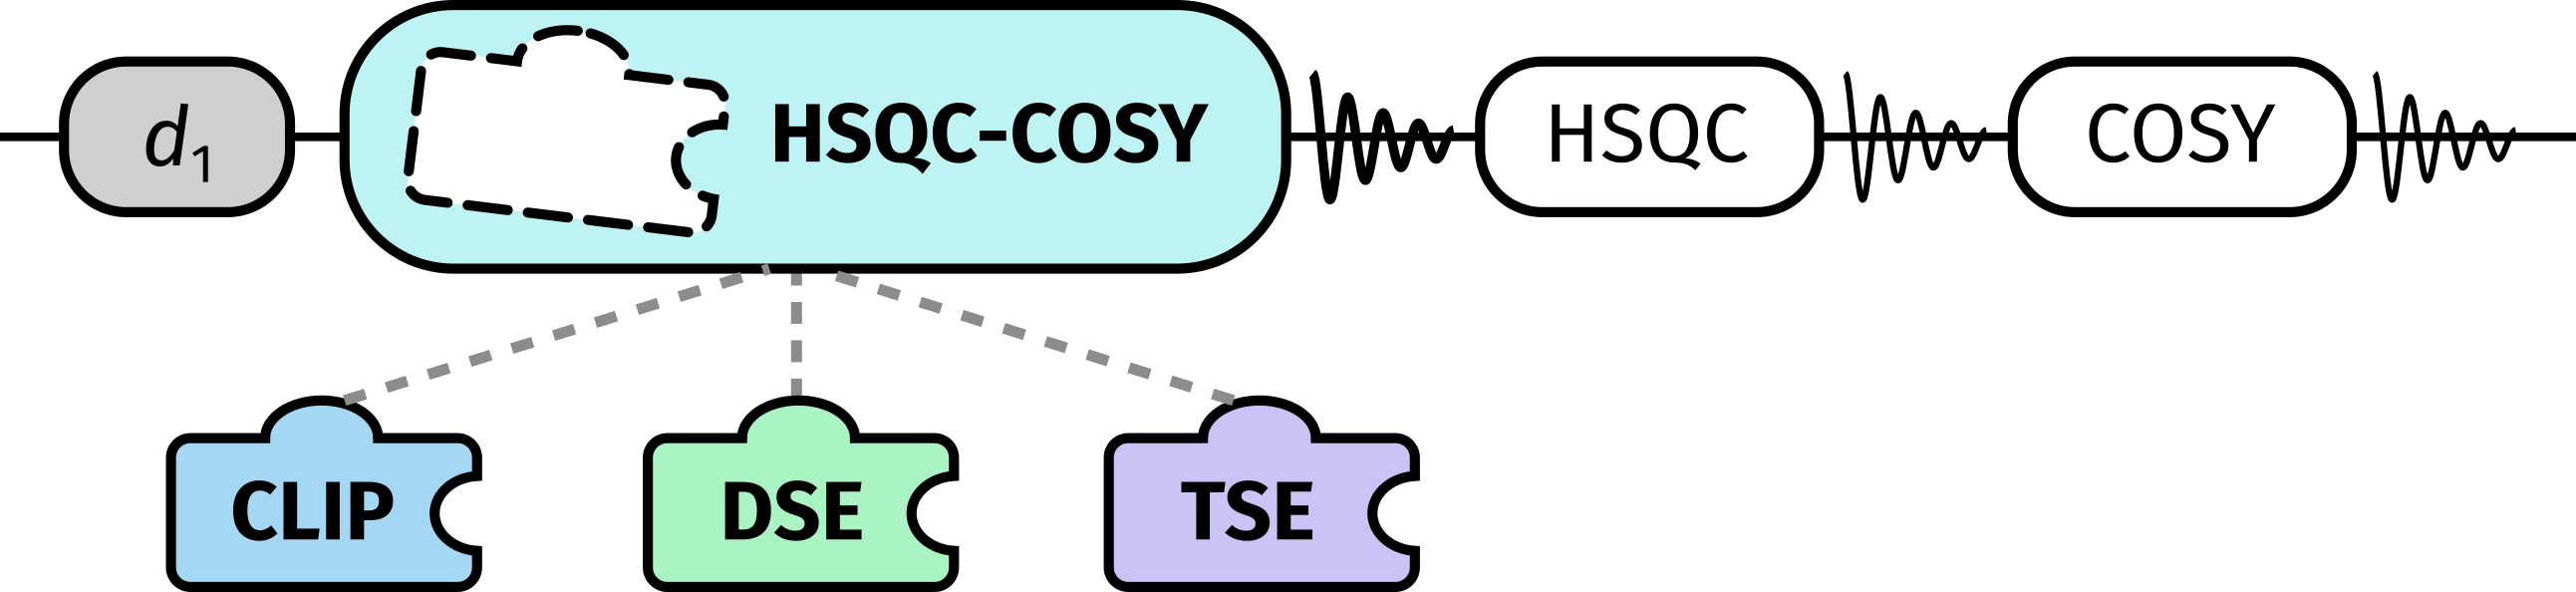
\includegraphics{toc.png}%
    \todo{TOC PIC GOES HERE}
\end{figure*}

\begin{itemize}
    \item Detailed discussion of HSQC-COSY implementations in NMR supersequences.
    \item Comparison of HSQC-COSY with HSQC-TOCSY.
    \item Sensitivity analyses of modules within typical NMR supersequences involving HSQC-COSY experiments.
\end{itemize}

NMR supersequences, as exemplified by the NOAH (NMR by Ordered Acquisition using \proton detection) technique, are a powerful way of acquiring multiple 2D data sets in much shorter durations.
This is accomplished through targeted excitation and detection of the magnetisation belonging to specific isotopologues (`magnetisation pools').
Separately, the HSQC-COSY experiment has recently seen an increase in popularity due to the high signal dispersion in the indirect dimension and the removal of ambiguity traditionally associated with HSQC-TOCSY experiments.
Here, we describe how the HSQC-COSY experiment can be integrated as a `module' within NOAH supersequences.
The benefits and drawbacks of several different pulse sequence implementations are discussed, with a particular focus on how sensitivities of other modules in the same supersequence are affected.

\clearpage

\section{Introduction}

The acceleration of multidimensional NMR spectroscopy has been an extremely popular topic in recent years, with techniques ranging from ultrafast NMR\autocite{Frydman2002PNASUSA,Pelupessy2003JACS,Frydman2003JACS} and non-uniform sampling (NUS)\autocite{Kazimierczuk2010PNMRS,Mobli2014PNMRS,Kazimierczuk2015MRC} to multiple-receiver technology\autocite{Kupce2006JACS,Kupce2008JACS,Kovacs2016MRC} and reduction of recovery delays\autocite{Kupce2007MRC,SchulzeSunninghausen2014JACS,Becker2019JMR}.
NOAH (NMR by Ordered Acquisition using \proton{} detection) experiments\autocite{Kupce2017ACIE}, which fall under the category of multiple-FID experiments\autocite{Yong2023RSCBook}, concatenate multiple 2D experiments (`modules') into a single nested pulse sequence with elision of intermediate recovery delays.
Such `supersequences' provide up to $4\times$ time savings compared to conventional, one-by-one acquisition of each 2D spectrum, and have gained popularity due to their versatility as well as the fact that they do not require specialised hardware.

\begin{figure}[!ht]
    \centering
    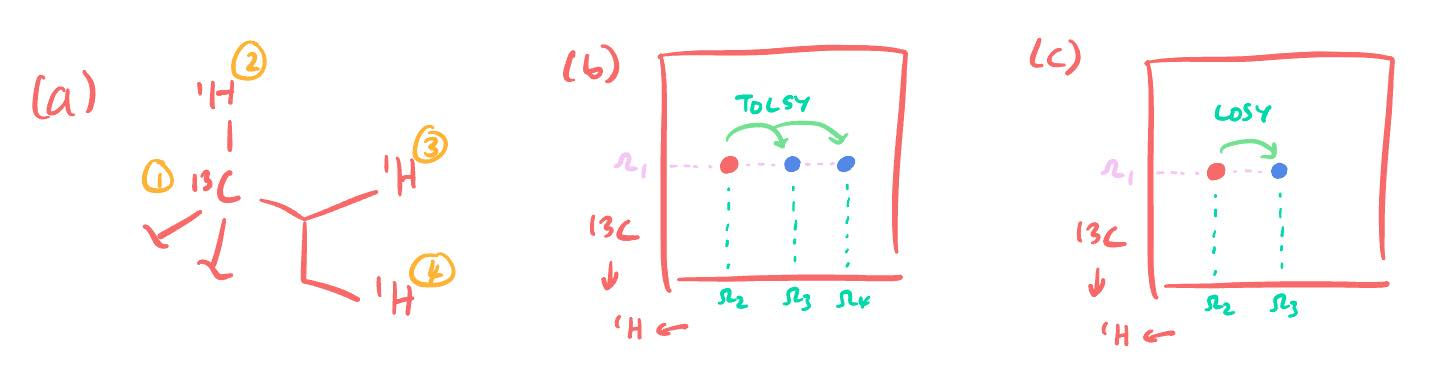
\includegraphics[width=\textwidth]{intro.jpg}%
    {\phantomsubcaption\label{fig:intro_molecular_structure}}%
    {\phantomsubcaption\label{fig:intro_hsqc_tocsy}}%
    {\phantomsubcaption\label{fig:intro_hsqc_cosy}}%
    \caption[Mockup illustrating salient features of HSQC-TOCSY and -COSY spectra]{
        \textbf{(\subref*{fig:intro_molecular_structure})} A typical fragment of an organic molecule, with one \carbon{} and three \proton{} spins.
        \textbf{(\subref*{fig:intro_hsqc_tocsy})} The corresponding HSQC-TOCSY spectrum. The `direct' peak at $(\Omega_1, \Omega_2)$ is shown in red, and the `indirect' peaks at $(\Omega_1, \Omega_3)$ and $(\Omega_1, \Omega_4)$ in blue: these have different signs due to an `editing' spin echo described later in the text.
        \textbf{(\subref*{fig:intro_hsqc_tocsy})} The corresponding HSQC-COSY spectrum, which is similar to the HSQC-TOCSY spectrum, except that there is only one `indirect' peak which arises from coherence transfer over ${}^3\!J_{\ch{HH}}$.
    }
    \label{fig:intro}
\end{figure}

Virtually all of the most commonly used 2D experiments have been adapted for use within NOAH supersequences, as neatly listed on the GENESIS website\autocite{Yong2022AC}.
In particular, we have previously described the implementation of the HSQC-TOCSY module in NOAH supersequences.\autocite{Yong2021JMR}
The HSQC-TOCSY experiment is extremely information-rich, providing both `direct' responses which arise from directly bonded \CH{} pairs, and `indirect' responses from protons in the same spin system as those bound to \carbon{} (\cref{fig:intro_molecular_structure,fig:intro_hsqc_tocsy})
This is essentially the same information as in separate HSQC and TOCSY spectra, but with the additional benefit that the TOCSY signals are dispersed more widely across the \carbon{} indirect dimension: this serves to greatly reduce the possibility of overlap and thus increase interpretability.

One downside of the HSQC-TOCSY is the largely indiscriminate transfer of magnetisation effected by the isotropic mixing block, which means that it is difficult to determine with certainty the number of bonds separating the \carbon{} and \proton{} resonances in the `indirect' responses.
A direct method of overcoming this is to instead record an HSQC-COSY spectrum, where the `indirect' responses arise only from single-step coherence transfer between directly coupled \HH{} pairs (\cref{fig:intro_hsqc_cosy}).
Experiments of this kind date back almost two decades, including the celebrated H2BC experiment\autocite{Nyberg2005JACS,Nyberg2005MRC}, and later 2BOB/H2OBC\autocite{Kupce2017MRC} and HMQC-COSY\autocite{Hu2011JBNMR}.
The 2BOB experiment in particular has previously been incorporated in NOAH supersequences\autocite{Kupce2019JMR}.
Since then, the HSQC-CLIP-COSY\autocite{Gyongyosi2018CPC,Gyongyosi2021AC} has emerged as a modern and improved experiment for this purpose: it provides pure absorption-mode lineshapes and does not suffer from amplitude modulation due to proton--proton couplings, a downside of the constant-time technique used in some of its predecessors.

Although the HSQC-CLIP-COSY performs admirably as a standalone experiment, the requirements for NOAH supersequences are more stringent: in particular, any HSQC-COSY module should---ideally---preserve unused magnetisation for later modules.
The most important example of this is magnetisation of all protons not directly bound to \carbon{} (denoted\autocite{Orts2018M,Yong2021JMR} `\magnnot{C}').
The HSQC-COSY module does not use this `magnetisation pool', and if it returns this magnetisation to the equilibrium $+z$ position, it can be sampled in a homonuclear module later in the supersequence.
Another key feature of the NOAH HSQC-TOCSY module is the fact that it allows for variable excitation of \carbon{}--bound proton magnetisation (denoted `\magn{C}'), meaning that a portion of it can be saved for a later heteronuclear module (e.g.\ an HSQC).
This feature was directly inspired by the ASAP-HMQC\autocite{Kupce2007MRC} and HSQC\autocite{SchulzeSunninghausen2014JACS,SchulzeSunninghausen2017JMR,Koos2019JMR,Becker2019JMR} sequences, which store partial \magn{C} magnetisation for subsequent $t_1$ increments instead of different modules.
We should therefore like any implementation of the HSQC-COSY to also exhibit this flexibility, as it allows the user to fine-tune the sensitivities of the modules within the supersequence for maximal performance.

In this work, we evaluate three different implementations of the NOAH HSQC-COSY module against several different criteria.
These pulse sequences have been very briefly described in our previous work, but in a different context of `parallel' supersequences\autocite{Kupce2021JACSA}: here we go into substantially more depth about the development, and the relative merits of, the three different HSQC-COSY forms.


\section{HSQC-CLIP-COSY}

\begin{figure}[!ht]
    \centering
    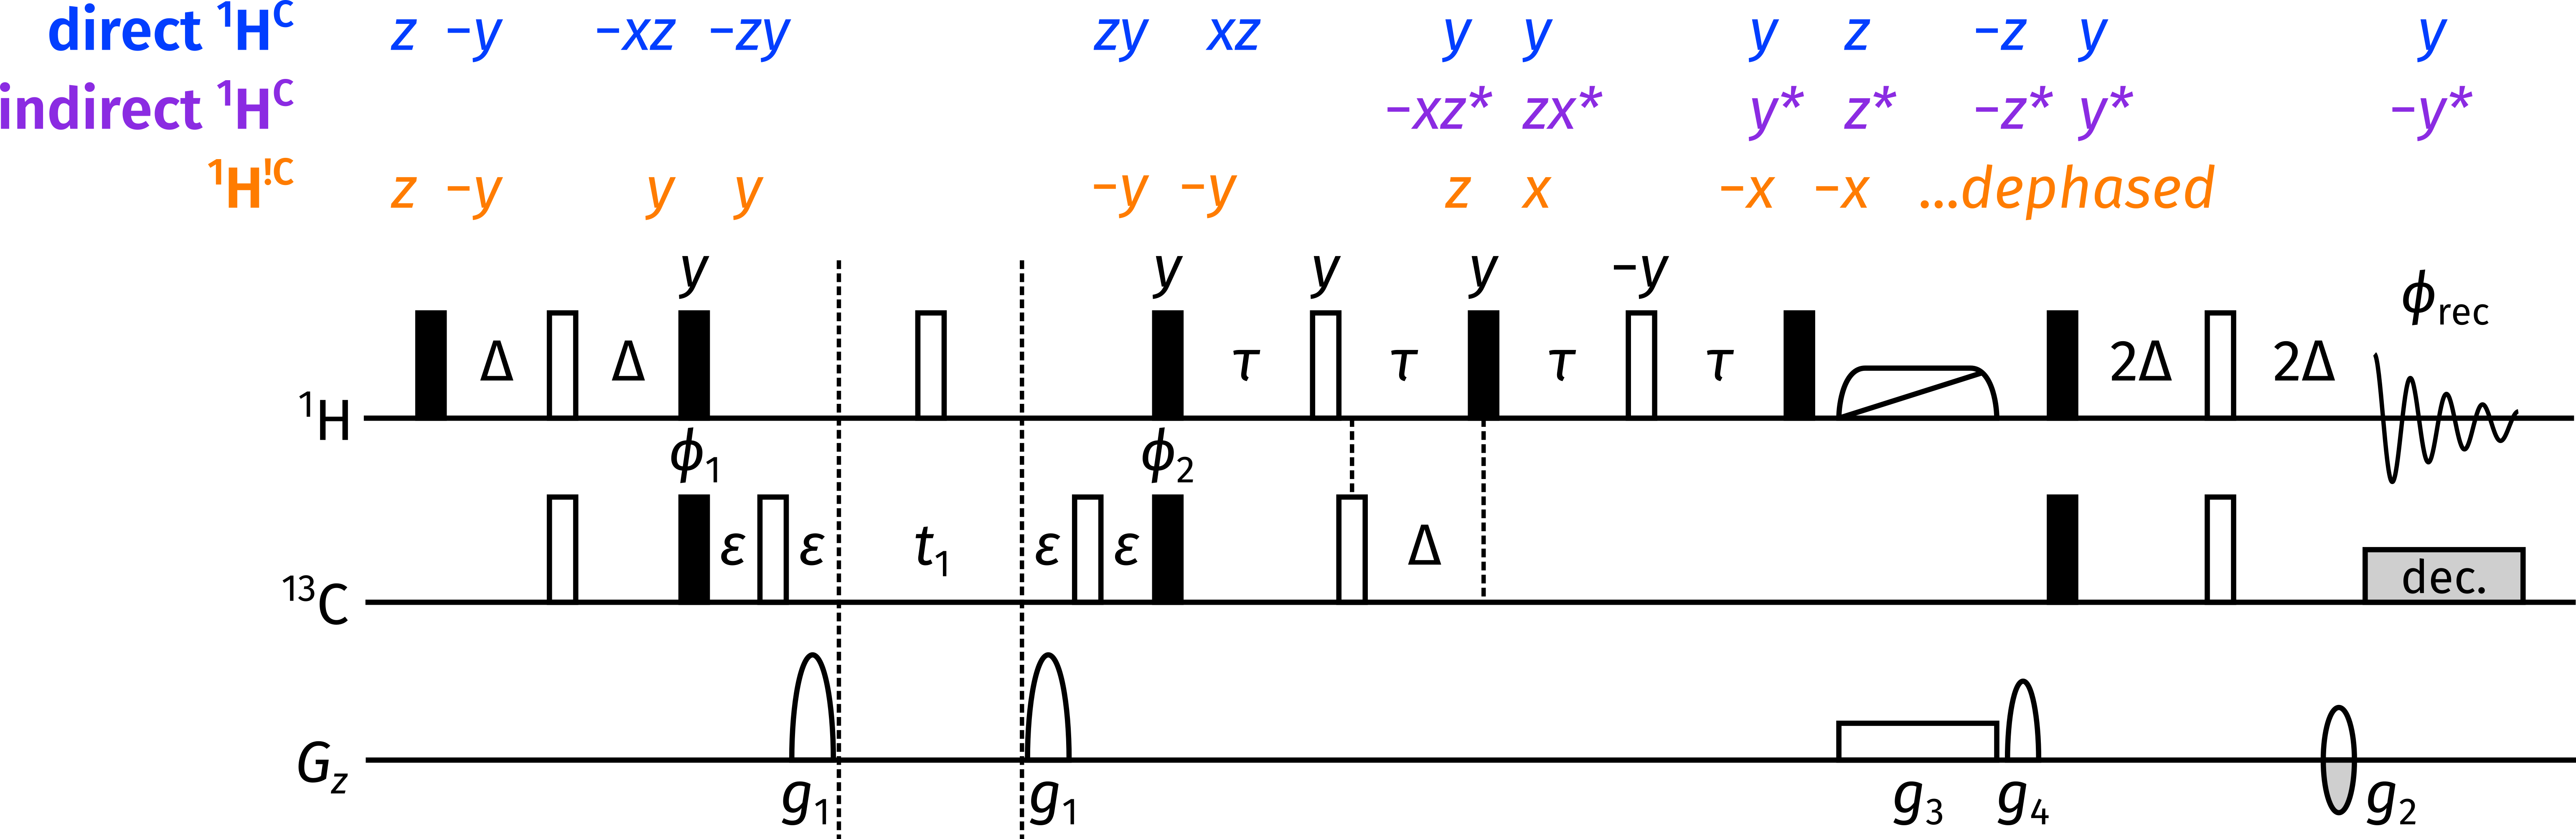
\includegraphics[]{clip_po.png}%
    \caption[HSQC-CLIP-COSY experiment]{
        HSQC-CLIP-COSY experiment with product operator analysis for a three-spin $ISR$ system, where $I$ is \carbon{}, $S$ is a directly bonded \proton{}, and $R$ a remote proton.
        Spins $I$ and $S$ are connected via one-bond \CH{} scalar coupling, and $S$ and $R$ via a (typically three-bond) \HH{} scalar coupling.
        Product operator analysis is provided for three relevant magnetisation pools: the `direct \magn{C}' HSQC-type peaks, the `indirect \magn{C}' responses which arise from coherence transfer from $S$ to $R$ in the perfect echo block, and the `\magnnot{C}' bulk magnetisation which we seek to preserve.
        Single-letter terms are shorthand for magnetisation on spin $S$ (for example, $x$ represents $S_x$); double-element terms to magnetisation on spins $I$ and $S$ (for example, $xz$ is $2I_xS_z$).
        Letters with asterisks refer to magnetisation on the remote spin $R$; thus, for example, $y^*$ means $R_y$, and $xz^*$ means $2I_xR_z$.
        Solid bars are \ang{90} pulses and empty bars \ang{180} pulses; the rounded trapezoid and line represent an adiabatic inversion pulse.
        All pulses are applied along the $+x$-axis unless otherwise specified; the symbolic pulse phases are $\phi_1 = (x, -x)$; $\phi_2 = (x, x, -x, -x)$; and $\phi_{\text{rec}} = (x, -x, -x, x)$.
        Pulsed field gradient amplitudes are $g_1 = \qty{37.10}{\gauss\per\cm}$ and $g_2 = \qty{18.66}{\gauss\per\cm}$.
        The gradient $g_3$ should be calibrated as per Thrippleton et al.\autocite{Thrippleton2003ACIE}; $g_4$ is a purge gradient with arbitrary amplitude.
        The delays $\Delta$ and $\tau$ are chosen to be $1 / (4 \cdot \oneJ{CH})$ and $1 / (4 \cdot \sum \nJ{HH})$; typically, $\oneJ{CH}$ and $\sum \nJ{HH}$ are respectively set as \qty{145}{\Hz} and \qty{30}{\Hz}, leading to values of $\Delta = \qty{1.72}{\ms}$ and $\tau = \qty{8.33}{\ms}$.
        $\varepsilon$ is the minimum time required for a pulsed field gradient plus a gradient recovery delay.
    }
    \label{fig:hsqcc_clip_po}
\end{figure}

The first implementation is the direct usage of the HSQC-CLIP-COSY sequence as a NOAH module (\cref{fig:hsqcc_clip_po}).
In this sequence, a standard HSQC experiment is supplemented with a clean in-phase (CLIP) coherence transfer block, formed from a perfect echo\autocite{Aguilar2012CC,Parella2019MRC,Koos2016ACIE} and a zero-quantum filter\autocite{Thrippleton2003ACIE} (\cref{fig:hsqcc_clip_po}).
The spin echo of duration $4\Delta$ just prior to detection allows for evolution of $\oneJ{CH}$, meaning that the `direct' responses acquire a negative sign, as illustrated in \cref{fig:intro_hsqc_cosy}.
Because of this inversion of direct responses, additional multiplicity editing in the HSQC step would lead to confusing spectra: thus, although the pulse sequences available on GENESIS do allow for multiplicity editing via an optional flag, they are omitted in the discussion which follows.

\begin{figure}[!htp]
    \centering
    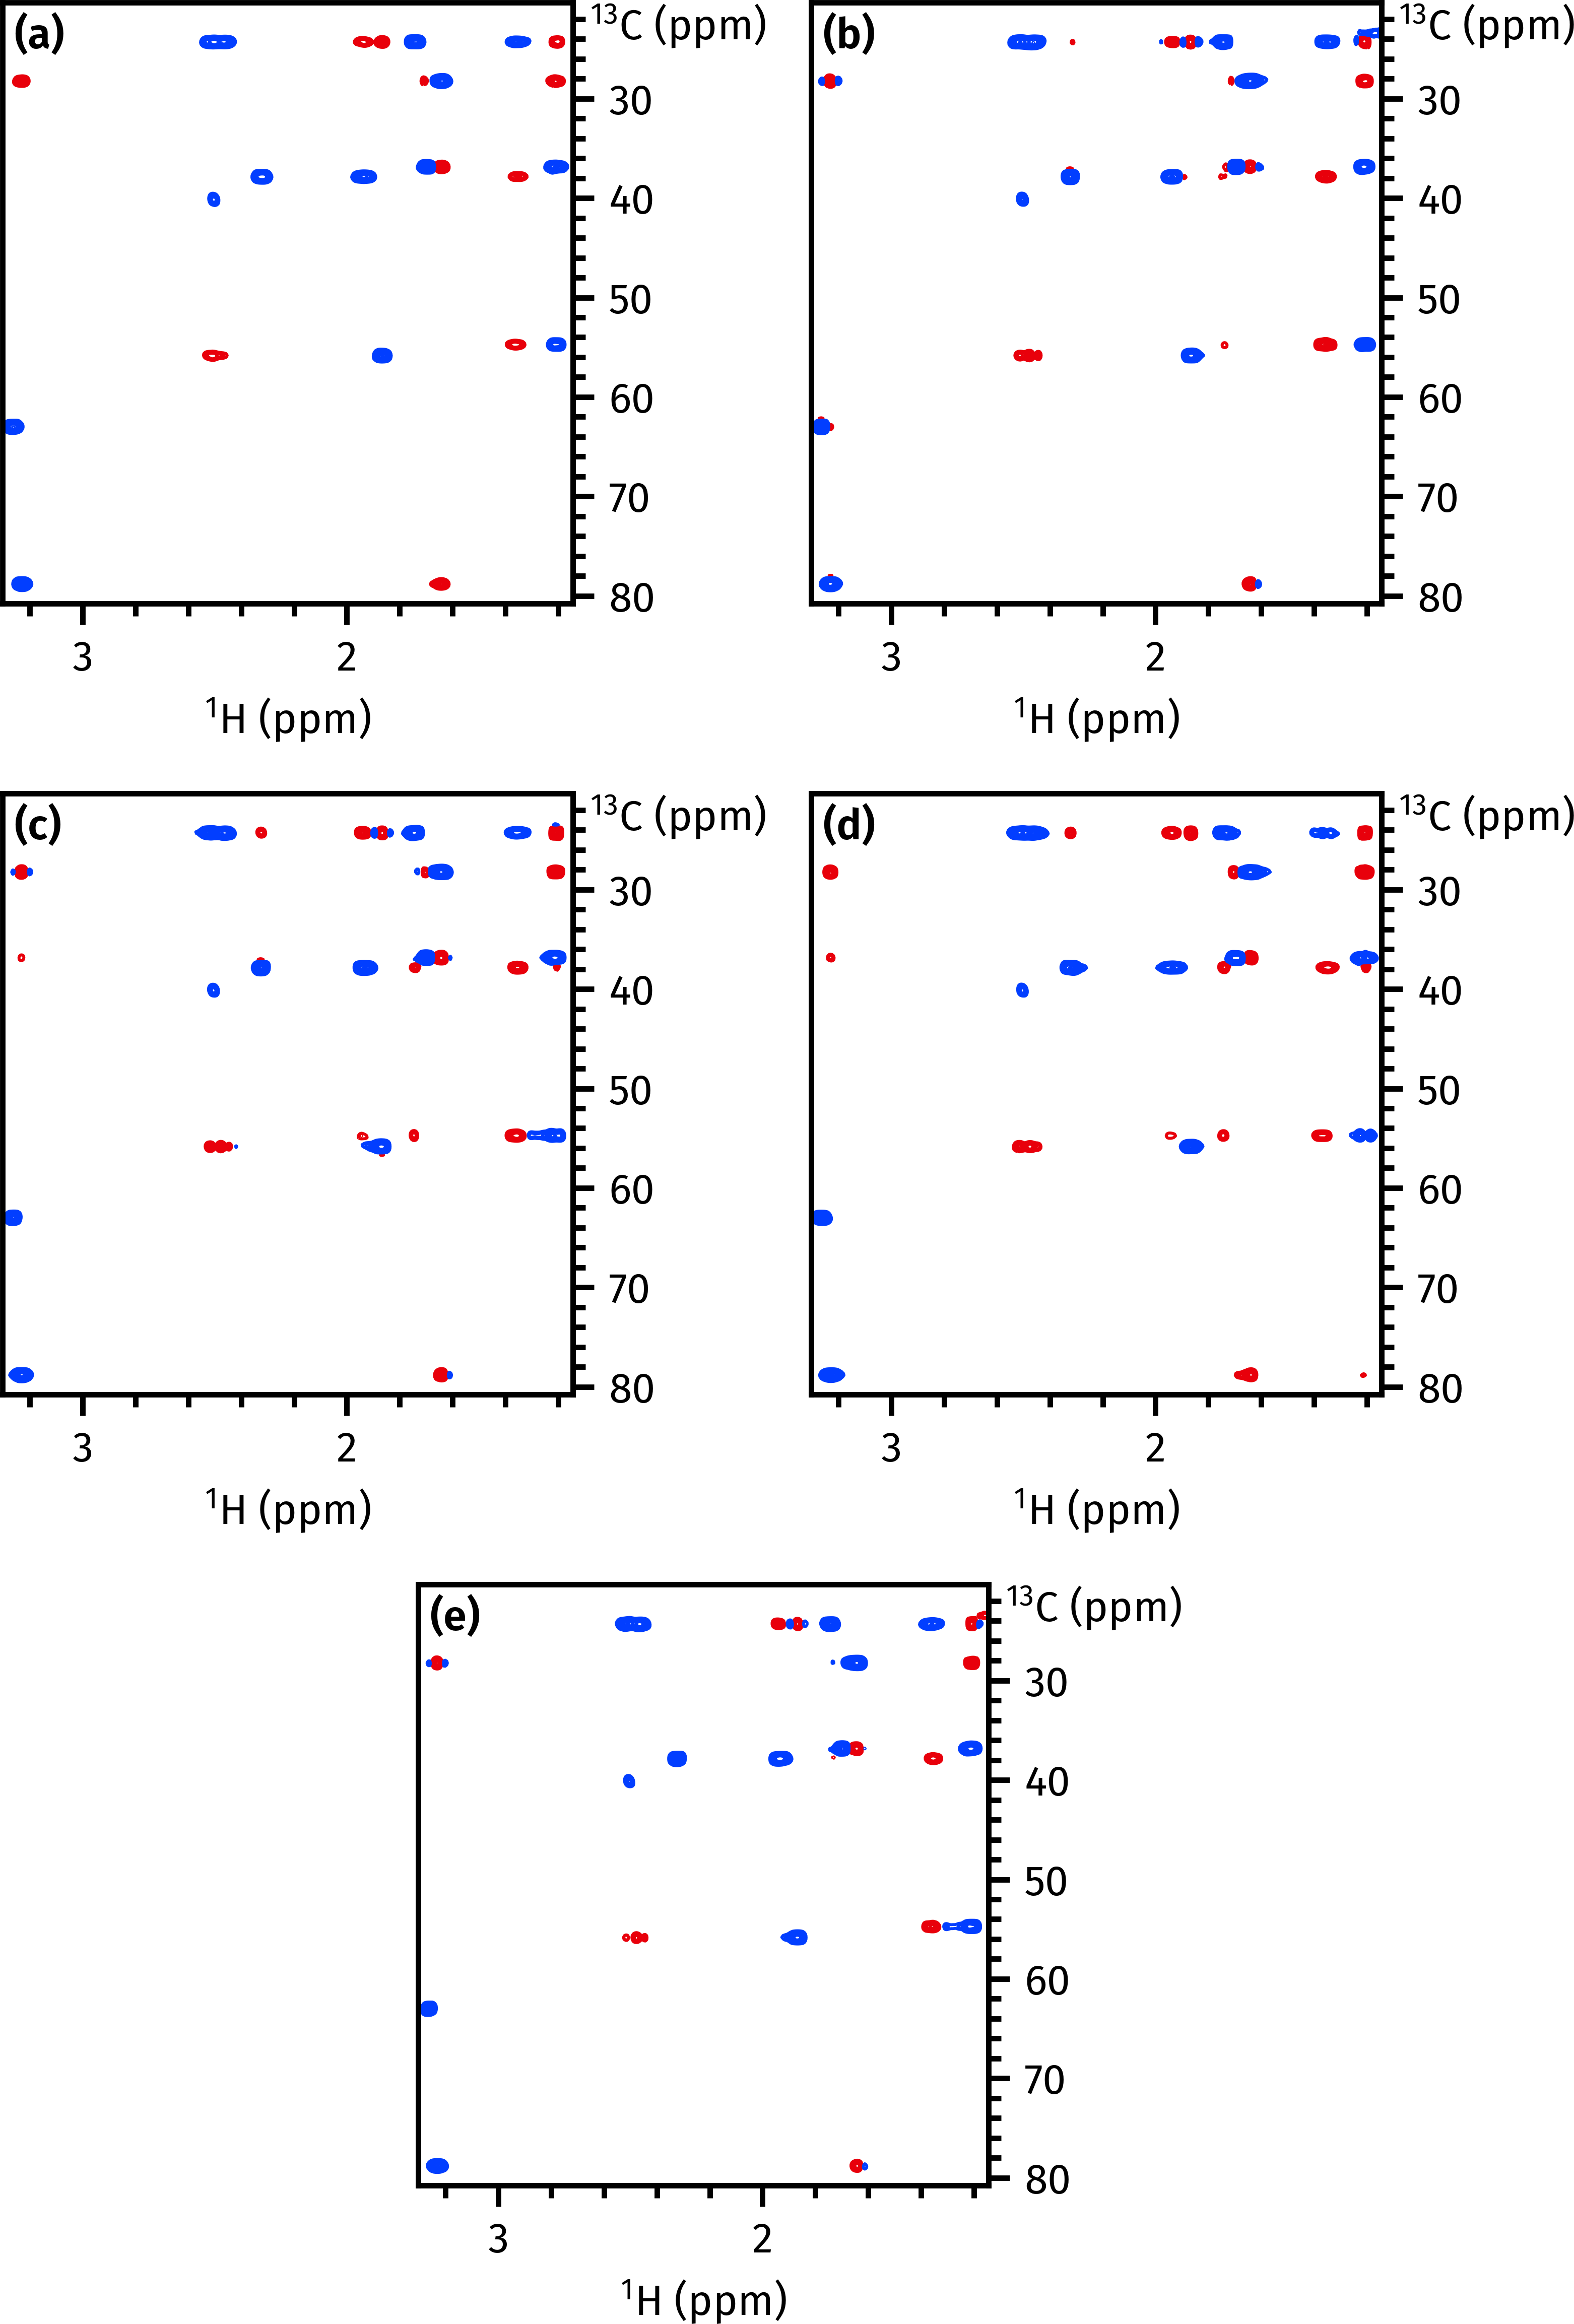
\includegraphics[]{hsqccosy_comp.png}%
    {\phantomsubcaption\label{fig:hsqccosy_comp_clip}}%
    {\phantomsubcaption\label{fig:hsqccosy_comp_dse}}%
    {\phantomsubcaption\label{fig:hsqccosy_comp_tse_norps}}%
    {\phantomsubcaption\label{fig:hsqccosy_comp_tocsy}}%
    {\phantomsubcaption\label{fig:hsqccosy_comp_tse}}%
    \caption[Comparison of spectra acquired with different HSQC-COSY modules]{
        HSQC-COSY and HSQC-TOCSY spectra, taken from (respectively) \noah{Sc,S,Cc} and \noah{St,S,Cc} experiments.
        \textbf{(\subref*{fig:hsqccosy_comp_clip})} HSQC-CLIP-COSY.
        \textbf{(\subref*{fig:hsqccosy_comp_dse})} DSE HSQC-COSY.
        \textbf{(\subref*{fig:hsqccosy_comp_tse_norps})} TSE HSQC-COSY without suppression of relay artefacts (described in the text).
        \textbf{(\subref*{fig:hsqccosy_comp_tocsy})} HSQC-TOCSY with \qty{10}{\ms} mixing time.
        \textbf{(\subref*{fig:hsqccosy_comp_tse})} TSE HSQC-COSY with suppression of relay artefacts.
        \andro{}
    }
    \label{fig:hsqccosy_comp}
\end{figure}

\begin{figure}[!ht]
    \centering
    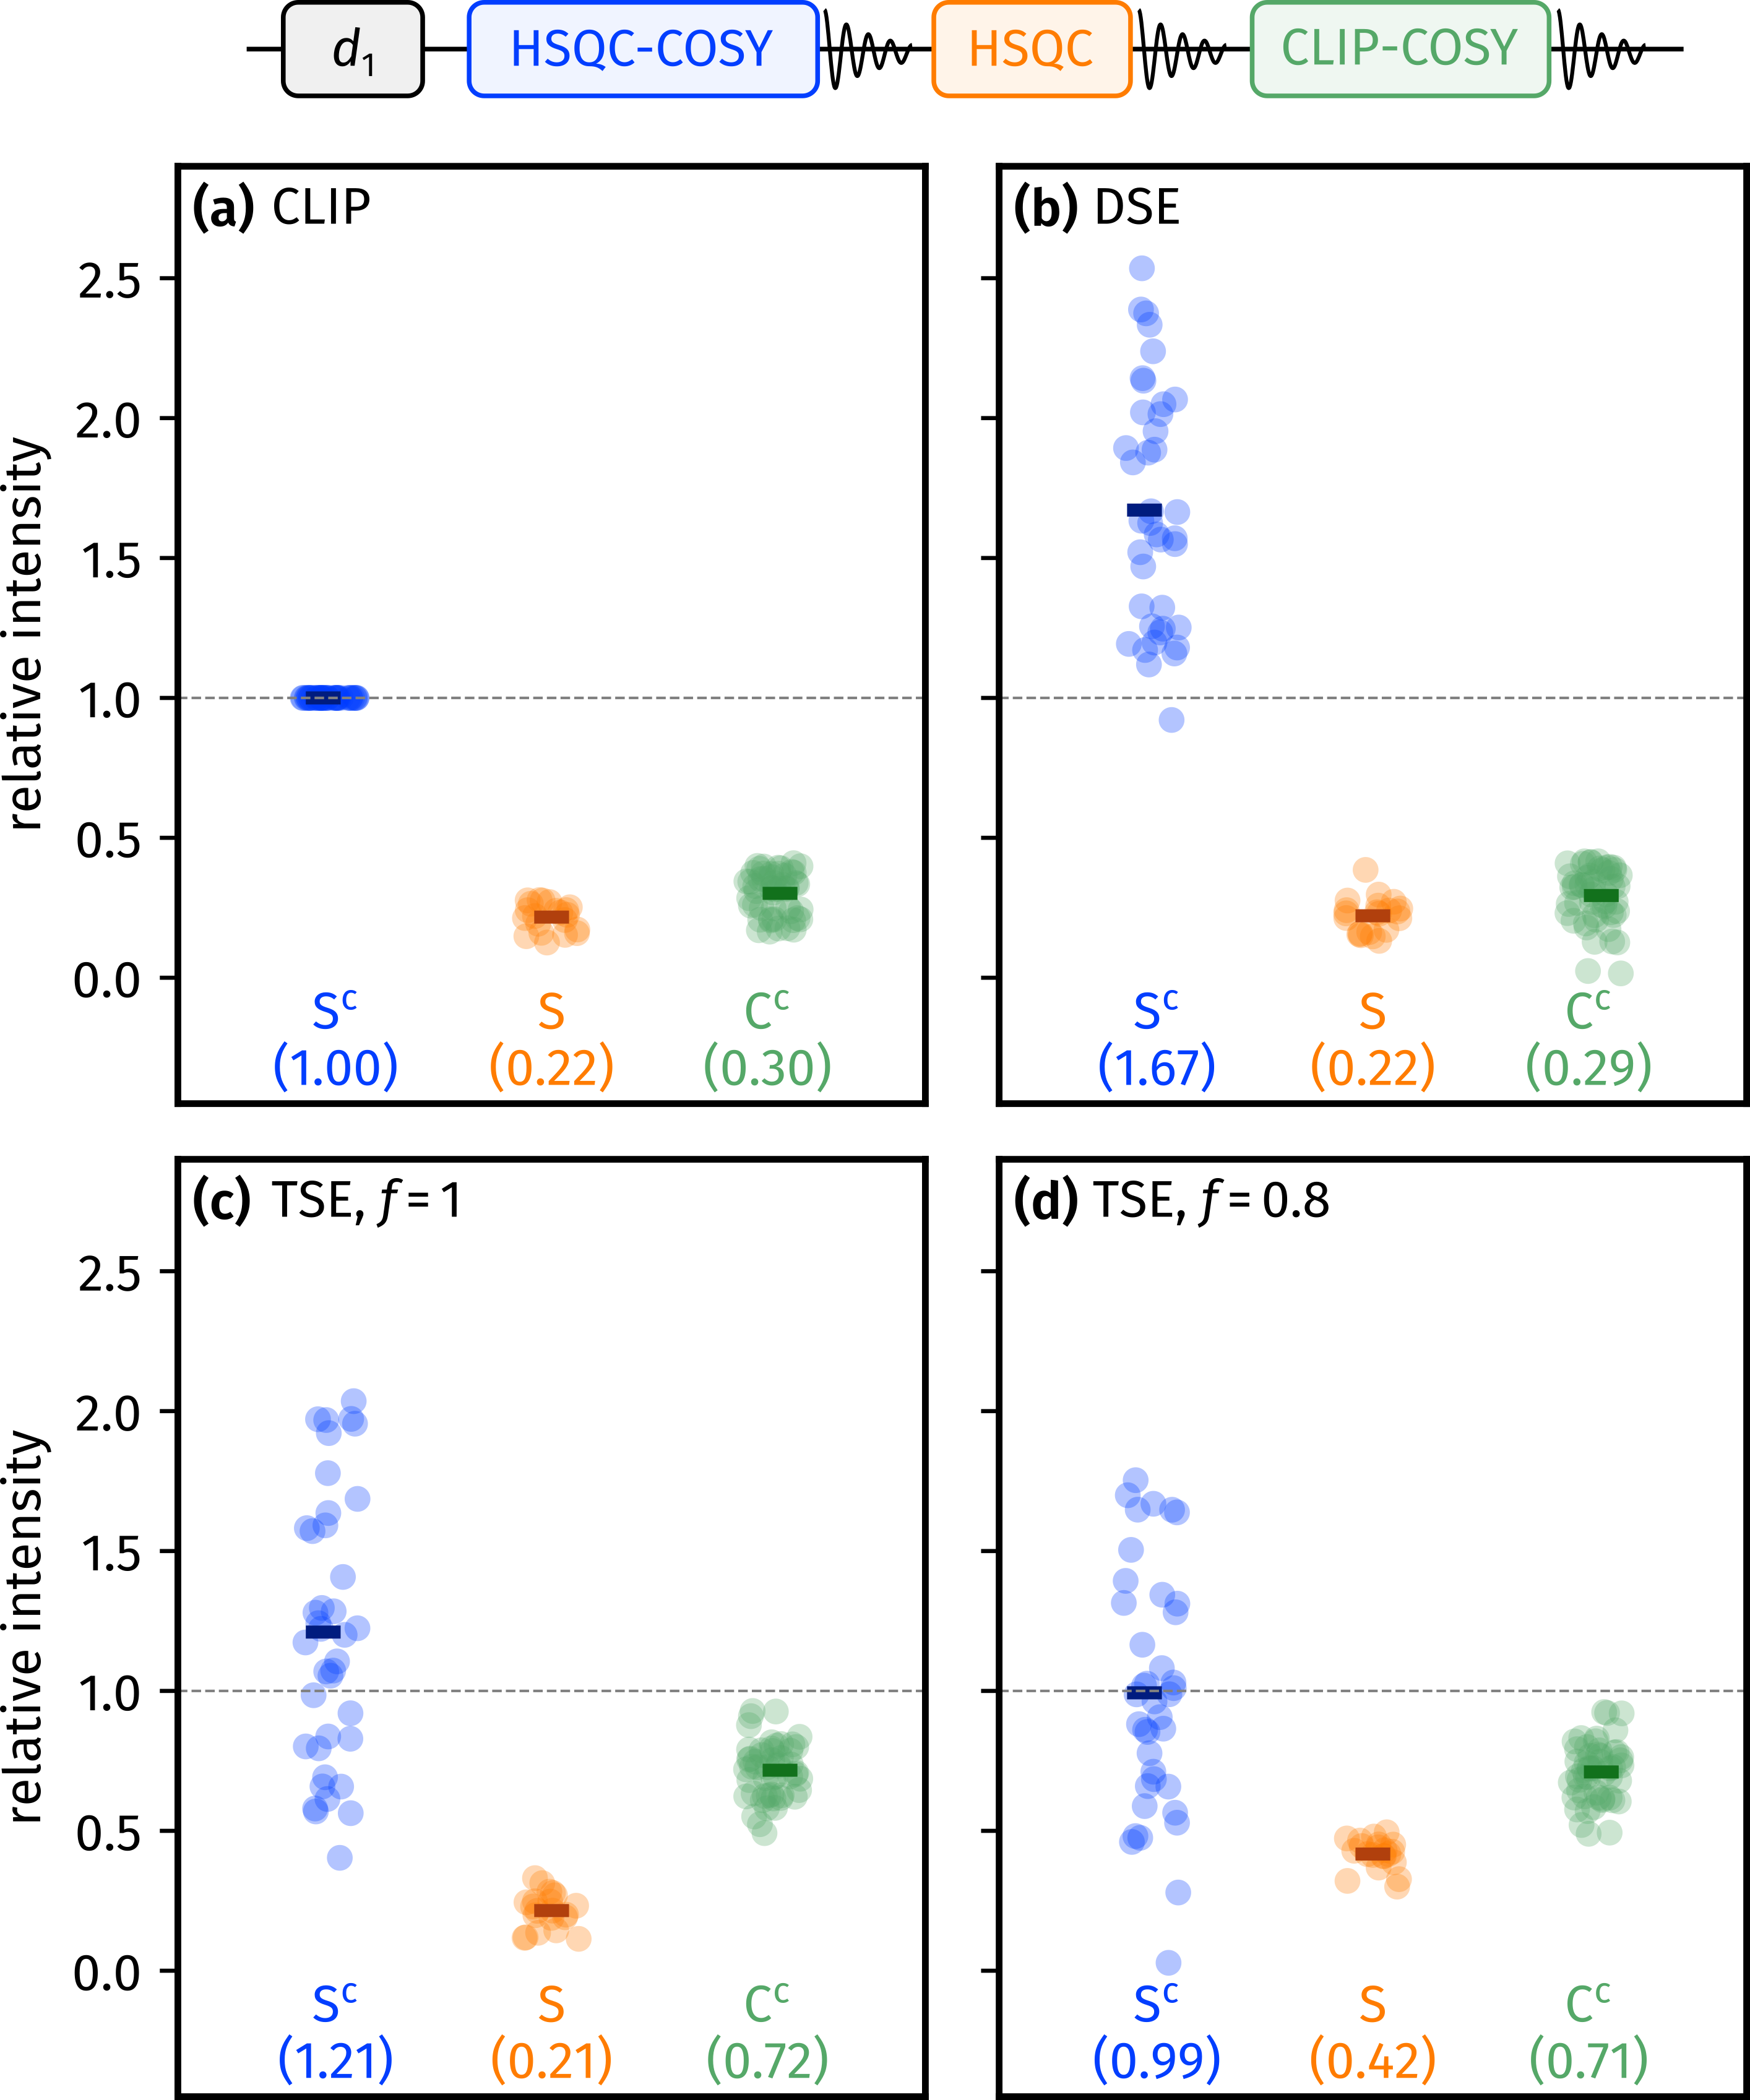
\includegraphics[]{hsqccosy_sens.png}%
    {\phantomsubcaption\label{fig:hsqccosy_sens_clip}}%
    {\phantomsubcaption\label{fig:hsqccosy_sens_dse}}%
    {\phantomsubcaption\label{fig:hsqccosy_sens_tse_1}}%
    {\phantomsubcaption\label{fig:hsqccosy_sens_tse_0p8}}%
    \caption[Sensitivity comparisons for \noah{Sc,S,Cc} supersequences]{
        \todo{(Insert schematic of NOAH supersequence.)}
        Sensitivity comparisons for all three modules in \noah{Sc,S,Cc} (HSQC-COSY + HSQC + CLIP-COSY) supersequences, using a variety of implementations for the HSQC-COSY module.
        Peak intensities of the first module are measured relative to the HSQC-CLIP-COSY module itself (the leftmost column in (\subref*{fig:hsqccosy_sens_clip})); whereas peak intensities of the HSQC and CLIP-COSY modules are measured relative to a separate, reference, \noah{S,Cc} experiment.
        Numbers in parentheses indicate averages over all peaks.
        \textbf{(\subref*{fig:hsqccosy_sens_clip})} HSQC-CLIP-COSY.
        \textbf{(\subref*{fig:hsqccosy_sens_dse})} DSE HSQC-COSY.
        \textbf{(\subref*{fig:hsqccosy_sens_tse_1})} TSE HSQC-COSY, acquired with $f = 1$.
        \textbf{(\subref*{fig:hsqccosy_sens_tse_0p8})} TSE HSQC-COSY, acquired with $f = 0.8$.
        \andro{}
    }
    \label{fig:hsqccosy_sens}
\end{figure}

The main benefit of the HSQC-CLIP-COSY sequence is the pure absorption-mode lineshapes yielded by the CLIP transfer (\cref{fig:hsqccosy_comp_clip}).
In this regard, it is the clear winner of all the sequences explored in this paper, as all the others generate a mixture of in-phase absorption and antiphase dispersion lineshapes.
However, this comes at a price: there is no way for this sequence to preserve any magnetisation for later modules, as the product operator analysis shows: all unused magnetisation is dephased by the end of the sequence.

It is reasonable to question whether minor adjustments can be made to the pulse sequence to render it NOAH-compatible, as has previously been done for modules such as HMBC\autocite{Claridge2019MRC,Kupce2019JMR} and sensitivity-enhanced HSQC\autocite{Hansen2021AC,Yong2021JMR}.
However, unfortunately, the CLIP element is wholly incompatible with preservation of unused magnetisation.
Specifically, the zero-quantum filter dephases any magnetisation that is not along $\pm z$ at this time.
However, if the `bulk' \magnnot{C} magnetisation were to be placed along $\pm z$, there would be no way to later differentiate it from the `indirect \magn{C}' magnetisation, since neither of these evolve under $\oneJ{CH}$.
Similar considerations preclude the possibility of variable \magn{C} excitation: if we had a portion of unused \magn{C} magnetisation that was intended to be stored for a subsequent module, this would have to be placed along the $z$-axis during the zero-quantum filter, but it cannot then be disentangled from the `direct \magn{C}' component which we do intend to detect.

A typical example of a NOAH supersequence featuring the HSQC-COSY module is a \noah{Sc,S,Cc} supersequence (\todo{FIG 4A}; \noah*{Sc} = HSQC-COSY, \noah*{S} = HSQC, and \noah*{Cc} = CLIP-COSY).
From a practical perspective, the HSQC module can be configured to include, for example, multiplicity editing or coupling in $F_2$, which provides additional information not present in the HSQC-COSY.
The CLIP-COSY module used here is simply a representative example of a homonuclear 2D spectrum which frequently terminates a NOAH supersequence: it can be replaced with (amongst others) NOESY, ROESY, TOCSY, or even a PSYCHE pure shift spectrum\autocite{Yong2022AC}.

In the present work, however, this supersequence is chosen to illustrate the effect of varying the HSQC-COSY implementation on downstream modules.
Because the HSQC-CLIP-COSY consumes all \magn{C} and \magnnot{C} magnetisation, both the HSQC and CLIP-COSY which come after it only sample magnetisation that has recovered during the acquisition periods interspersed between modules.
Thus, both of these modules have substantially reduced sensitivity (\cref{fig:hsqccosy_sens_clip}) when compared against a \noah{S,Cc} supersequence (i.e., the same supersequence but with the HSQC-COSY removed).


\section{Double spin echo HSQC-COSY}

\begin{figure}[!ht]
    \centering
    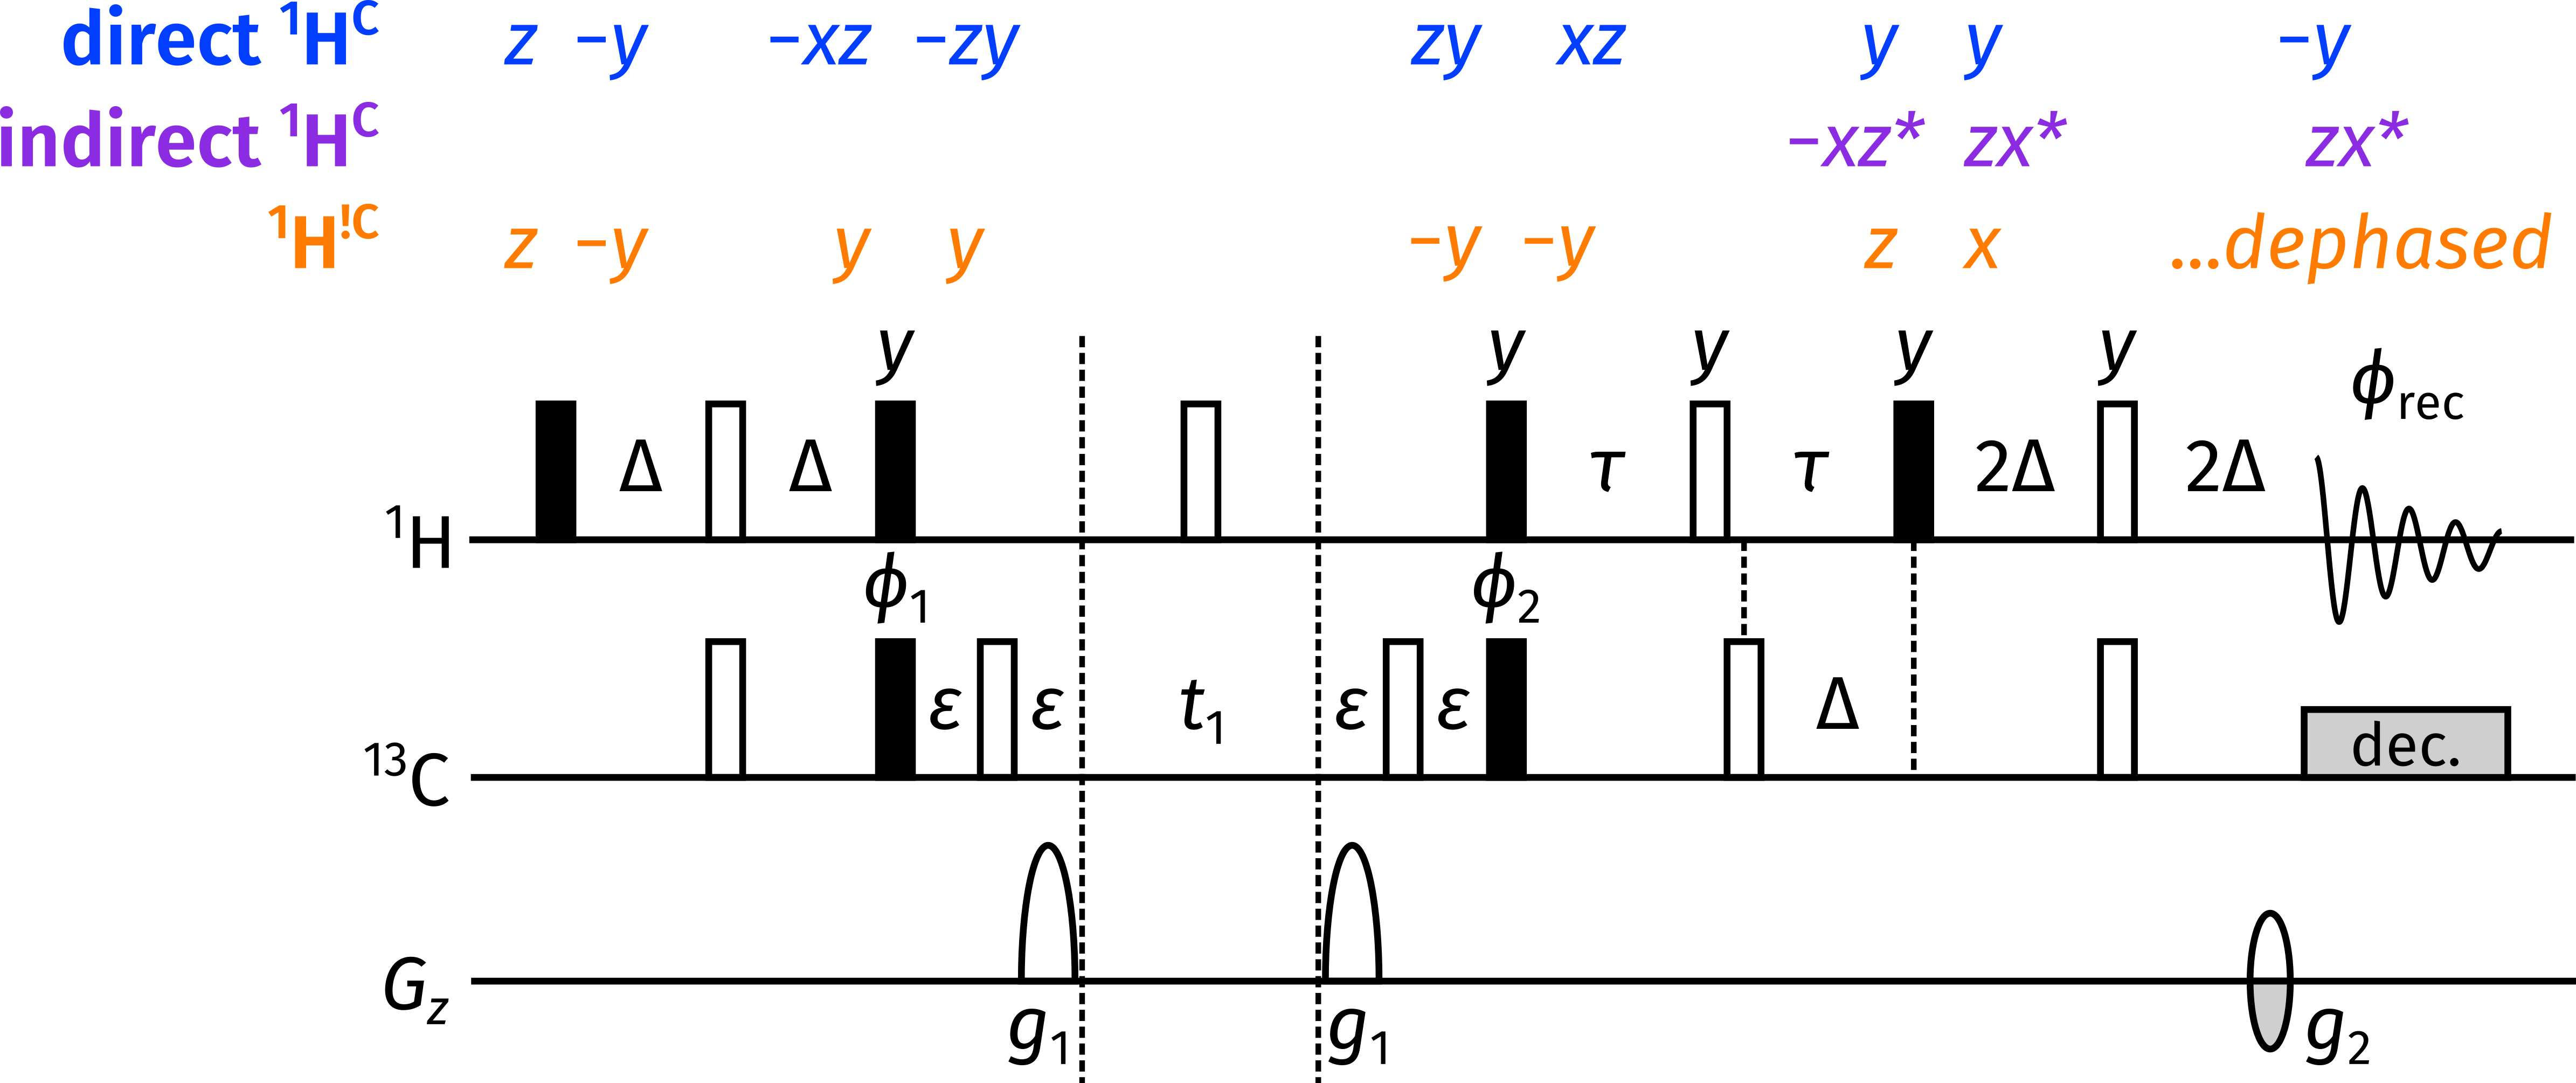
\includegraphics[]{dse_po.png}%
    \caption[Double spin echo HSQC-COSY experiment]{
        `Double spin echo' HSQC-COSY experiment; all symbols have the same meaning as in \cref{fig:hsqcc_clip_po}.
    }
    \label{fig:hsqcc_dse_po}
\end{figure}

The purpose of the CLIP element in the HSQC-CLIP-COSY is to effect coherence transfer from one proton to another proton coupled to it.
However, given that this CLIP element makes it impossible to preserve unused magnetisation, it is worth considering what happens when this is replaced with the simplest pulse sequence element for coherence transfer---namely, a spin echo followed by a \ang{90} pulse.
This simplification results in the `double spin echo' (DSE) HSQC-COSY, so-named because it has two spin echoes after the $t_1$ period (\cref{fig:hsqcc_dse_po}).

The removal of the CLIP element leads to mixed lineshapes in this experiment, where the direct responses are (mostly) in-phase absorption, and the indirect responses (mostly) antiphase dispersion.
This is clearly visible in the spectrum (\cref{fig:hsqccosy_comp_dse}): the antiphase dispersion components are visible as `wings' of opposite sign which flank each peak.
On the other hand, because the antiphase magnetisation generated during the spin echo is not purged, the DSE HSQC-COSY sequence provides the greatest sensitivity of all the HSQC-COSY implementations here: for the sample used here, it yielded (on average) a 60\% increase in sensitivity compared to the HSQC-CLIP-COSY.
Unfortunately, as before, the DSE experiment does not preserve bulk magnetisation; it is also incompatible with partial \magn{C} excitation.
Thus, the sensitivities of the subsequent modules in the \noah{Sc,S,Cc} supersequence remain very low (\cref{fig:hsqccosy_sens_dse}), and (accounting for noise) are identical to those seen previously with the HSQC-CLIP-COSY.

% It is worth mentioning here that the DSE HSQC-COSY has exactly the same effect on bulk magnetisation as a standard sensitivity-enhanced HSQC (seHSQC)\autocite{Kay1992JACS,Schleucher1994JBNMR}.
% Thus, prepending this DSE HSQC-COSY with the $zz$ isotope-selective pulse (ZIP) element would allow it to return the bulk \magnnot{C} magnetisation to $+z$ at the end of the sequence, as has previously been done for the NOAH seHSQC module\autocite{Hansen2021AC,Yong2021JMR}.
% However, this was not evaluated experimentally.

\section{Triple spin echo HSQC-COSY}

\begin{figure}[!ht]
    \centering
    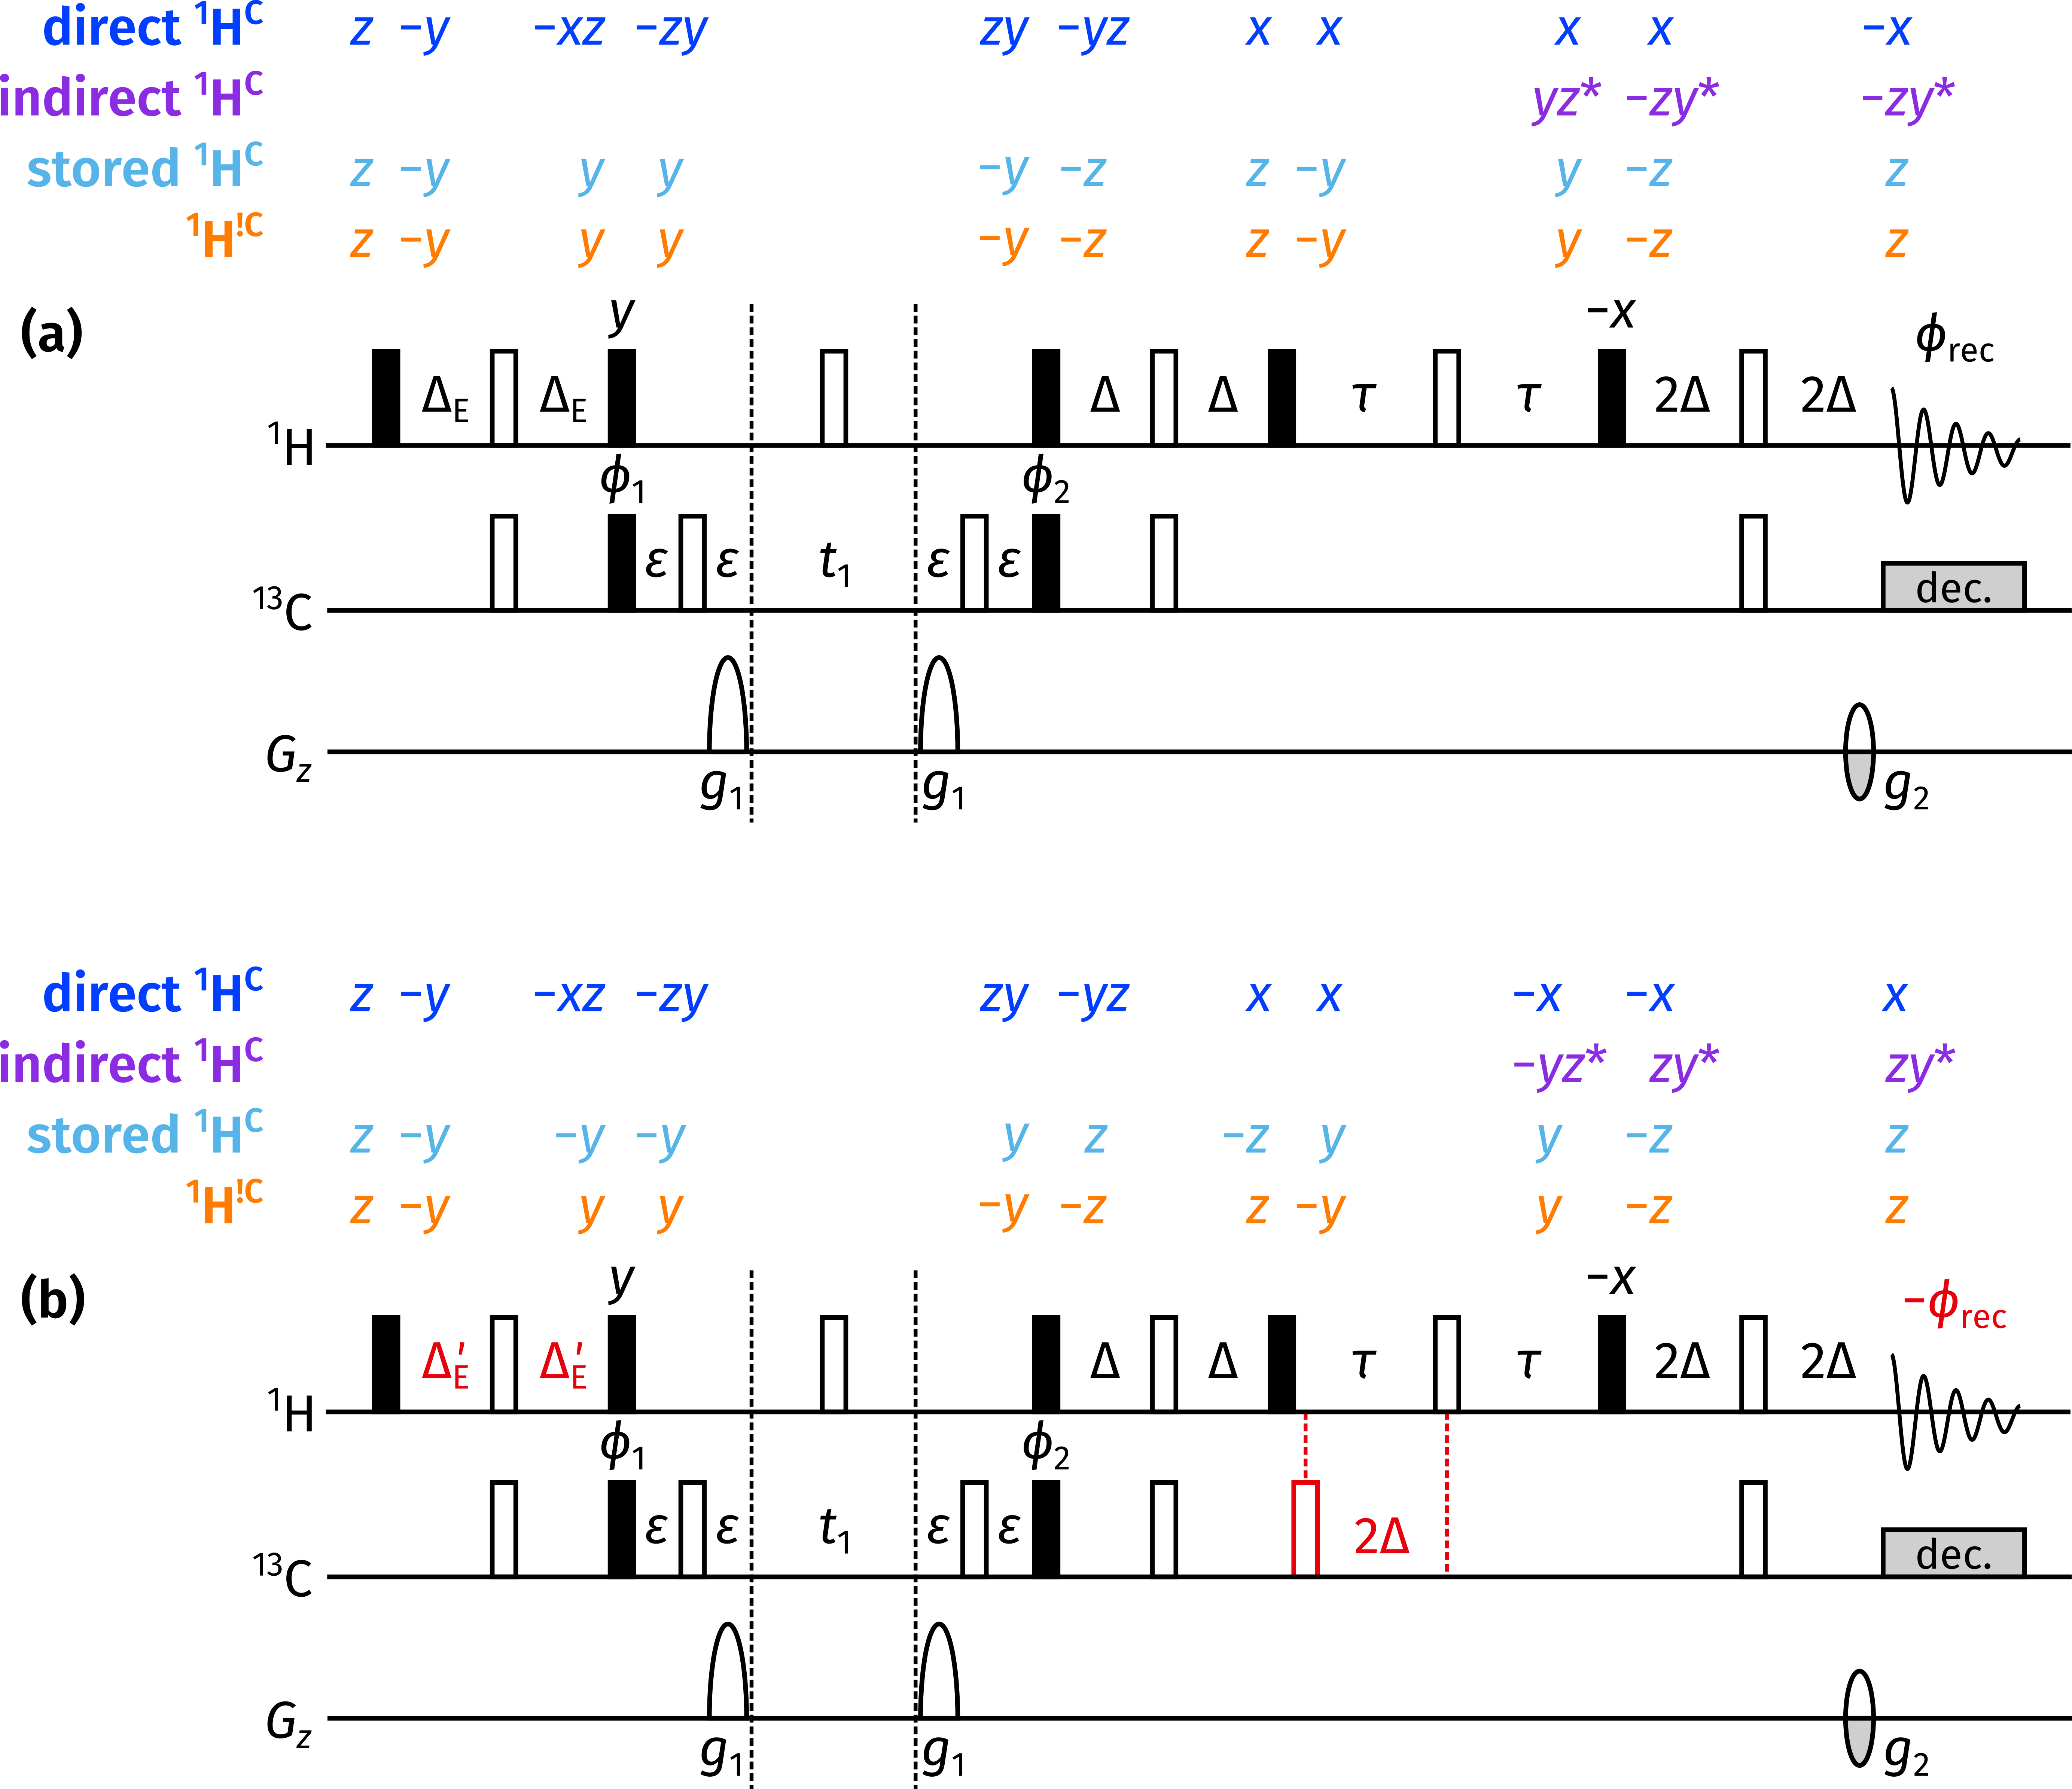
\includegraphics[]{tse_po.png}%
    {\phantomsubcaption\label{fig:hsqcc_tse_po_1}}%
    {\phantomsubcaption\label{fig:hsqcc_tse_po_2}}%
    \caption[Triple spin echo HSQC-COSY experiment]{
        `Triple spin echo' (TSE) HSQC-COSY experiment.
        \textbf{(\subref*{fig:hsqcc_tse_po_1})} The first part of the experiment; this can be used on its own, but leads to spurious `relayed' peaks arising via coherence transfer over two scalar couplings.
        The initial INEPT delay $\DeltaE$ can be adjusted so as to excite only a portion of the \magn{C} magnetisation pool: to excite a fraction $f \in [0, 1]$ of this magnetisation, $\DeltaE$ should be set to $(2\Delta \arcsin f)/\cpi$.
        \textbf{(\subref*{fig:hsqcc_tse_po_2})} The second part of the experiment; co-adding this dataset with the first part leads to suppression of the relayed peaks.
        Differences from (\subref*{fig:hsqcc_tse_po_1}) are highlighted in red: in particular, the value of $\DeltaE'$ should be $(2\Delta (\pi - \arcsin f))/\cpi$.
        All other symbols have the same meaning as in \cref{fig:hsqcc_clip_po}.
    }
    \label{fig:hsqcc_tse_po}
\end{figure}

As shown above, neither of the two HSQC-COSY implementations above (CLIP or DSE) can successfully preserve unused magnetisation.
The triple spin echo (TSE) HSQC-COSY was introduced to remedy this problem.
We first consider only the `basic', first part of the TSE HSQC-COSY (\cref{fig:hsqcc_tse_po_1}).
This pulse sequence differs from the DSE HSQC-COSY by the splitting up of the first of the two spin echoes after $t_1$ into two separate spin echoes: one of duration $2\Delta$ for $\oneJ{CH}$ refocusing, and one of duration $2\tau$ for $\nJ{HH}$ evolution.
This not only leads to preservation of the bulk \magnnot{C} magnetisation, but also enables partial \magn{C} excitation by shortening the delay $\Delta$ in the initial INEPT step to $\DeltaE$.
The product operators immediately after the second $\DeltaE$ delay are $\cos(2\cpi J_{IS} \DeltaE) I_y - \sin(2\cpi J_{IS} \DeltaE) 2I_xS_z$; thus, if we want to excite a proportion $f$ of \magn{C} magnetisation ($0 \leq f \leq 1$), we should set
$$f = \sin(2\cpi J_{IS} \DeltaE) \implies \DeltaE = \arcsin{f}/(2\cpi J_{IS}),$$
and since $\Delta = 1/(4J_{IS})$, we have that $\DeltaE = (2\Delta \arcsin{f}) / \cpi$.
This is identical to that previously described for the NOAH HSQC-TOCSY module\autocite{Yong2021JMR} (although a factor of $2/\cpi$ was erroneously omitted there).

While this sequence exhibits the desired behaviour in terms of magnetisation preservation, the introduction of one extra spin echo leads to the possibility of two-step coherence transfer through successive \HH{} couplings and thus spurious peaks.
In particular, the intensity of this unwanted transfer pathway is proportional to the extent to which $J_{SR}$ evolves during the first spin echo after $t_1$: therefore, these `relay' artefacts are especially prominent for large magnitudes of $J_{SR}$, such as $^2\!J$ or axial--axial $^3\!J$.
This is seen clearly in the resulting spectrum (\cref{fig:hsqccosy_comp_tse_norps}): a number of extra peaks are visible compared to the CLIP and DSE HSQC-COSY implementations.
Indeed, this naive implementation of the TSE HSQC-COSY very much resembles a HSQC-TOCSY acquired with a short mixing time (\cref{fig:hsqccosy_comp_tocsy}), which defeats the purpose of the HSQC-COSY experiment.

This drawback, however, can be elegantly addressed by the introduction of a second experiment (\cref{fig:hsqcc_tse_po_2}).
The most obvious difference here is the addition of a single \carbon{} \ang{180} pulse, highlighted in red.
This addition causes $\oneJ{CH}$ to evolve for a total duration of $4\Delta$ during the $2\tau$ spin echo, causing any magnetisation of \carbon{}--bound protons to be inverted.
Conversely, magnetisation which has already undergone coherence transfer to a remote proton during the preceding spin echo is not affected.
Thus, the effect is to invert the desired signal, while leaving the relay artefacts untouched.
Subtracting this second dataset from the first (or equivalently, as is done here, inverting the receiver phase on the second and then adding them together) leads to suppression of the relay artefacts.

A more subtle point is that the insertion of an extra \ang{180} pulse also causes any unexcited (i.e., stored) \magn{C} magnetisation to be inverted.
In order to ensure that this is returned to $+z$ at the end of the sequence, instead of $-z$, a slight adjustment must also be made to the INEPT delay for variable excitation: instead of being shortened, it must be lengthened to a value of $\DeltaE' = (2\Delta (\cpi - \arcsin f))/\cpi$, where as before $f$ is the fraction of \magn{C} magnetisation to be excited.

\todo{Talk about improvement in spectral quality resulting from this}

\todo{Talk about sensitivity of TSE HSQC-COSY compared to CLIP and DSE}

\todo{Note to self: sensitivity of no-suppression TSE version is meaningless as there are large spurious sensitivity increases due to double transfer pathways}

\todo{Talk about sensitivity of downstream modules}

\todo{Discuss sensitivity in supersequences with HMBC. I wonder, maybe this should go to the SI?}


\section*{Acknowledgements}

We thank Dr Mohammadali Foroozandeh (University of Oxford) for helpful discussions.
\meshort{}\ thanks the Clarendon Fund (University of Oxford) and the EPSRC Centre for Doctoral Training in Synthesis for Biology and Medicine (EP/L015838/1) for a studentship, generously supported by AstraZeneca, Diamond Light Source, Defence Science and Technology Laboratory, Evotec, GlaxoSmithKline, Janssen, Novartis, Pfizer, Syngenta, Takeda, UCB, and Vertex.

% Fakesection Bibliography
\AtNextBibliography{\small}
\printbibliography{}
\end{refsection}


% Fakesection ================= SI ==================

\clearpage
\begin{refsection}
\newcommand{\sectionbreak}{\clearpage}
\renewcommand*{\thefigure}{S\arabic{figure}}
\renewcommand*{\thesection}{S\arabic{section}}
\renewcommand*{\thetable}{S\arabic{table}}
\renewcommand*{\thepage}{S\arabic{page}}
\setcounter{page}{1}
\setcounter{figure}{0}
\setcounter{section}{0}
\setcounter{table}{0}
\onehalfspacing

\hspace{0pt}
\vfill
\begin{center}
    \huge
    Supporting Information

    \vspace{0.3cm}

    \textit{for}

    \vspace{0.3cm}

    \articletitle{}

    \vspace{0.6cm}

    \Large \me{},\textsuperscript{1} \eriks{},\textsuperscript{2} \tim{}\textsuperscript{1,\texttt{*}}

    \vspace{0.6cm}

    \large \textsuperscript{1} \textit{\crl{}}

    \textsuperscript{2} \textit{\brukeruk{}}

    \textsuperscript{\texttt{*}} \texttt{tim.claridge@chem.ox.ac.uk}

\end{center}
\vfill

\newpage
\section*{Contents}

\startcontents[si]
\printcontents[si]{ }{1}{}
\vfill
\hspace{0pt}
\newpage


\section{OLD STUFF FROM THESIS: Supersequence sensitivity}

\Cref{fig:hsqccosy_sens} also shows the relative sensitivities of the later modules in \noah{Sc,S,Cc} supersequences.
In all of the first three cases (CLIP, DSE, and TSE HSQC-COSY with $f = 1$, \cref{fig:hsqccosy_sens_clip,fig:hsqccosy_sens_dse,fig:hsqccosy_sens_tse_1}), the HSQC sensitivity is low (ca.\ 20\%) because no \magn{C} magnetisation is retained for it to use.
Thus, the signal derives only from \magn{C} magnetisation which has recovered during the HSQC-COSY FID.
However, when the TSE version is used, partial \magn{C} excitation can be used to control this sensitivity: for example, when $f = 0.8$ (\cref{fig:hsqccosy_sens_tse_0p8}), the HSQC-COSY sensitivity is decreased (on average equalling that of the HSQC-CLIP-COSY), but the sensitivity of the HSQC module is almost doubled.
Generally, choosing a value of $f < 1$ allows for the HSQC-COSY and HSQC sensitivities to be better balanced.

Finally, the CLIP-COSY module suffers when the HSQC-CLIP-COSY or the DSE HSQC-COSY are used, because both of these dephase \magnnot{C} magnetisation;
however, the TSE version successfully preserves around $70\%$ of this magnetisation for it, regardless of the value of $f$.
(This value is slightly lower than the approximately $90\%$ magnetisation preserved by the HSQC module, because the bulk magnetisation is placed in the transverse plane during the $2\tau$ spin echo (\cref{fig:hsqcc_tse_po_1}) and experiences losses due to $\nJ{HH}$ evolution.)


\section{OLD STUFF FROM THESIS: HSQC-COSY in context}

\begin{figure}[!ht]
    \centering
    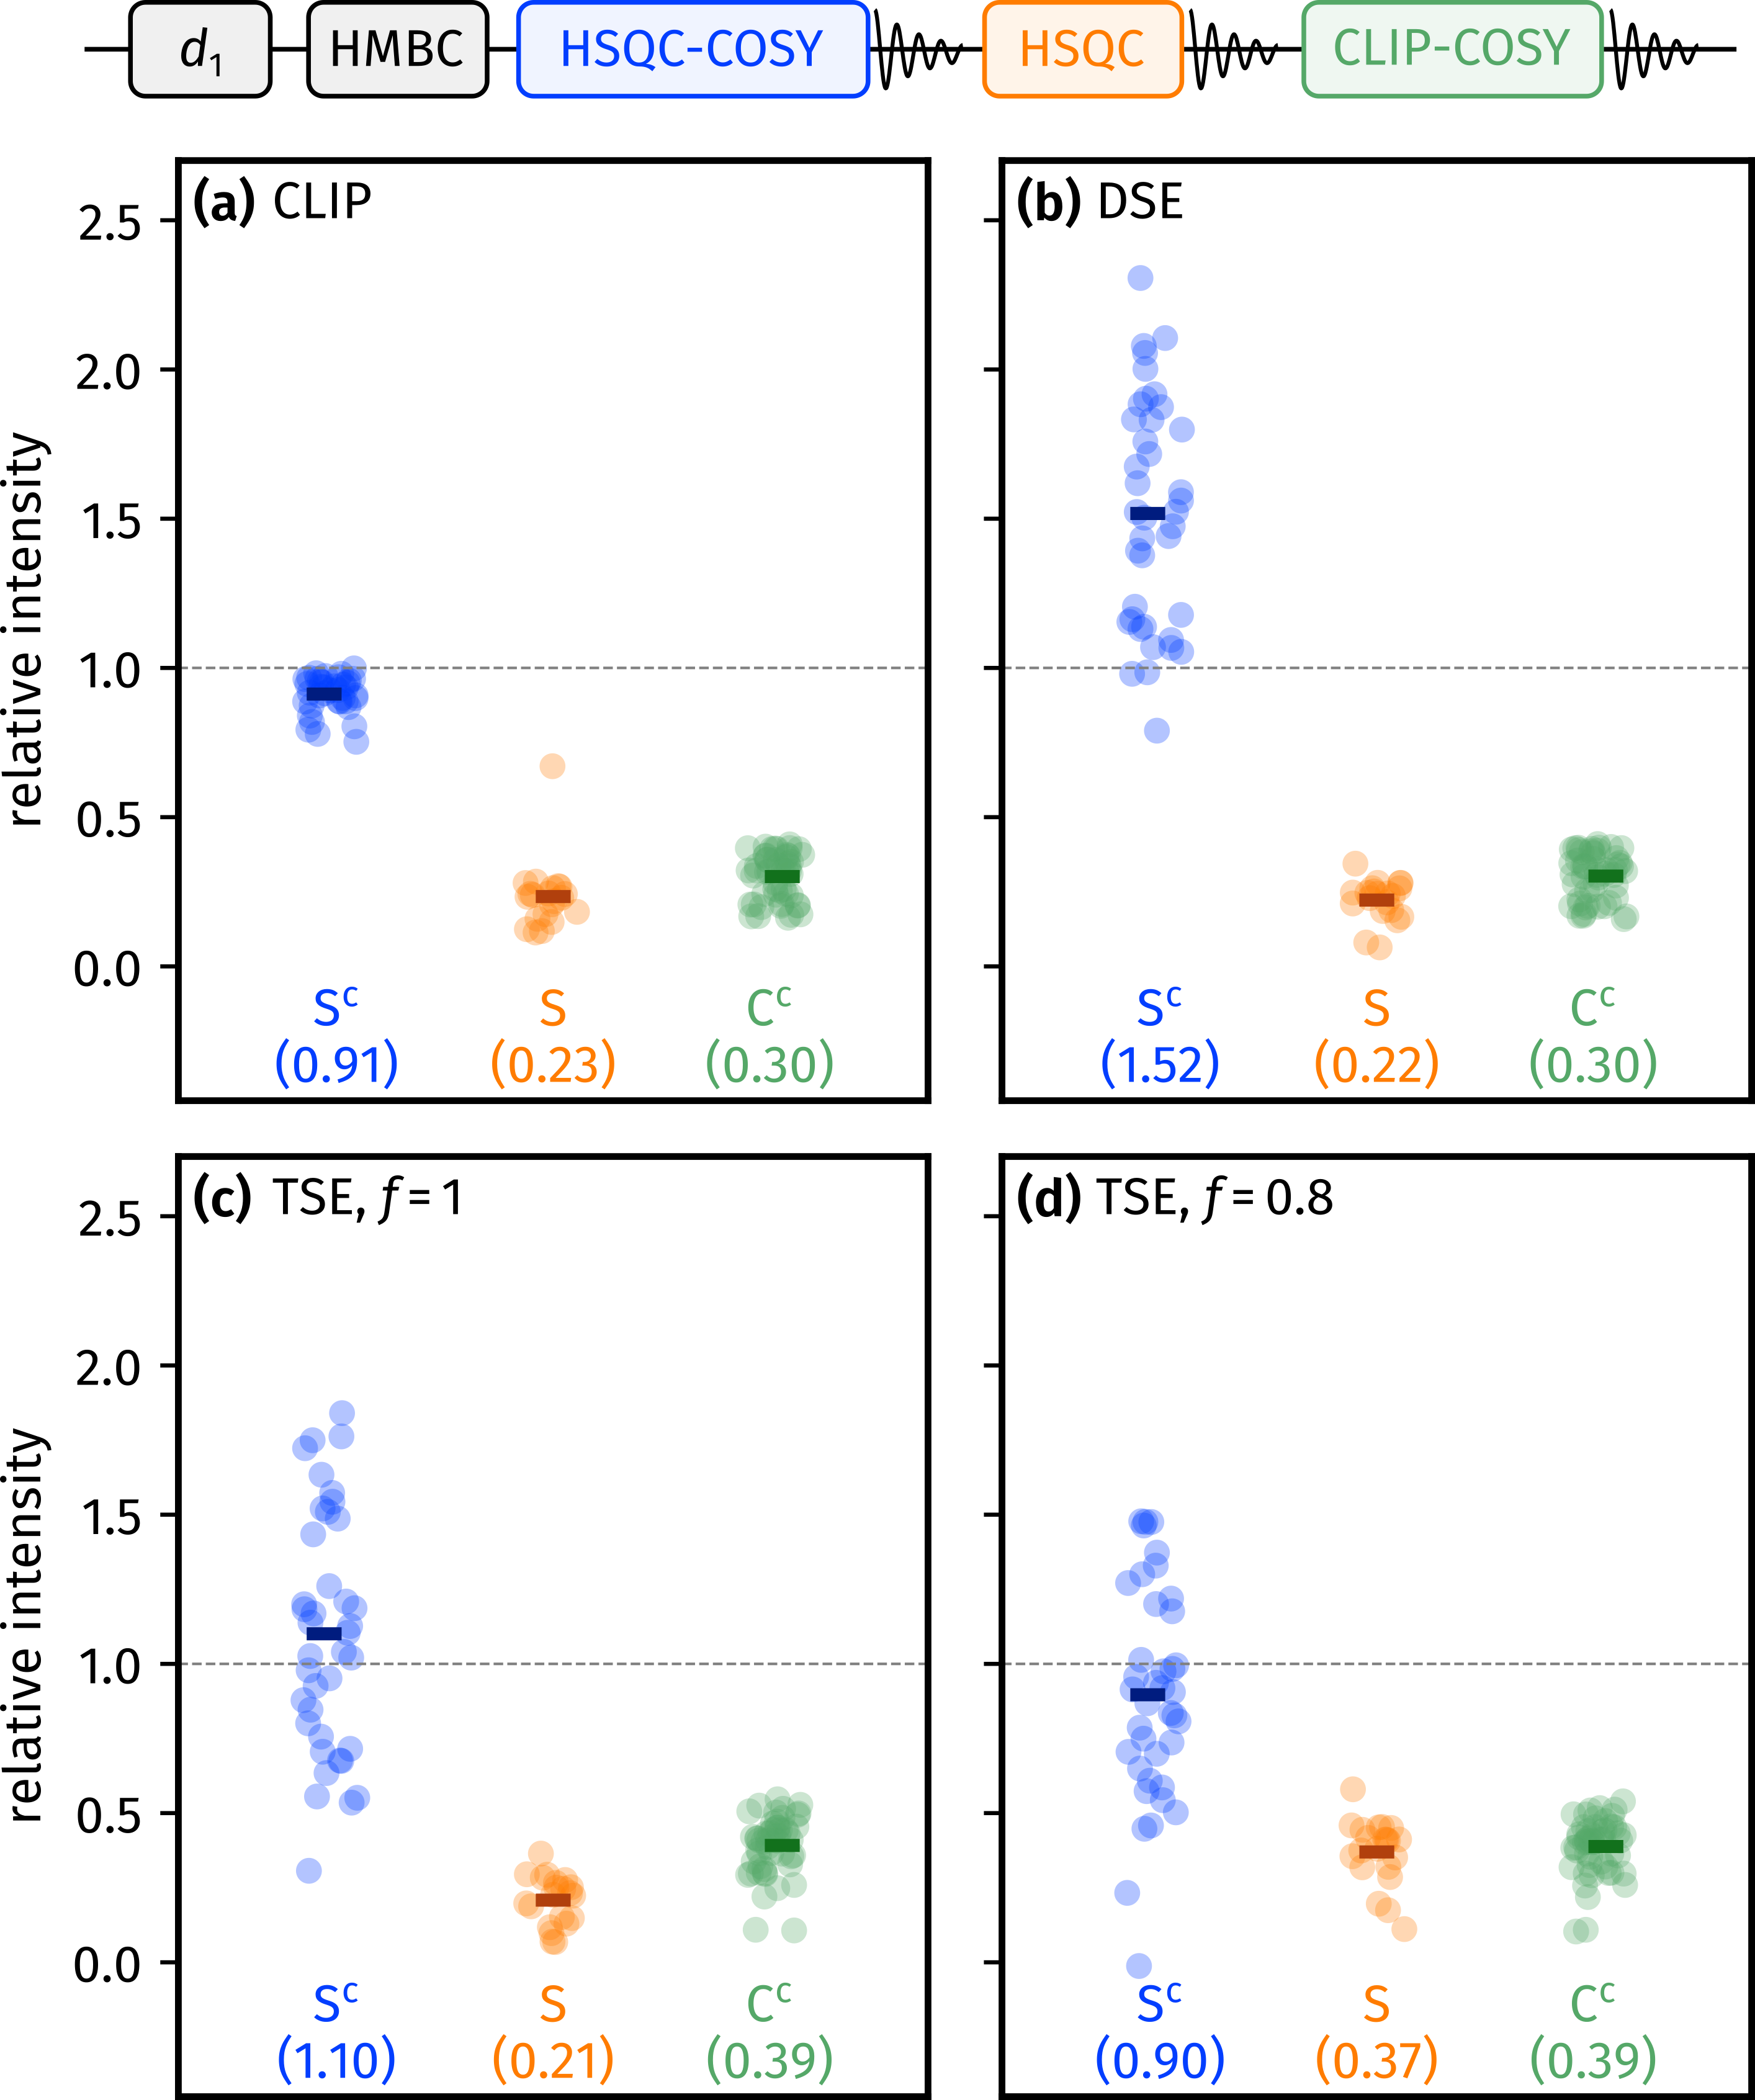
\includegraphics[]{hsqccosy_sens_with_hmbc.png}%
    {\phantomsubcaption\label{fig:hsqccosy_sens_with_hmbc_clip}}%
    {\phantomsubcaption\label{fig:hsqccosy_sens_with_hmbc_dse}}%
    {\phantomsubcaption\label{fig:hsqccosy_sens_with_hmbc_tse_1}}%
    {\phantomsubcaption\label{fig:hsqccosy_sens_with_hmbc_tse_0p8}}%
    \caption[Sensitivity comparisons for \noah{B,Sc,S,Cc} supersequences]{
        Sensitivity comparisons for the three last modules in \noah{B,Sc,S,Cc} supersequences.
        Peak intensities are relative to the HSQC-CLIP-COSY module from a \noah{Sc,S,Cc} supersequence, and HSQC and CLIP-COSY spectra from a \noah{S,Cc} experiment (these are the same reference spectra as used in \cref{fig:hsqccosy_sens}).
        Numbers in parentheses indicate averages over all peaks.
        \textbf{(\subref*{fig:hsqccosy_sens_with_hmbc_clip})} HSQC-CLIP-COSY.
        \textbf{(\subref*{fig:hsqccosy_sens_with_hmbc_dse})} DSE HSQC-COSY.
        \textbf{(\subref*{fig:hsqccosy_sens_with_hmbc_tse_1})} TSE HSQC-COSY, acquired with $f = 1$.
        \textbf{(\subref*{fig:hsqccosy_sens_with_hmbc_tse_0p8})} TSE HSQC-COSY, acquired with $f = 0.8$.
        7A-210723
    }
    \label{fig:hsqccosy_sens_with_hmbc}
\end{figure}

In \noah{Sc,S,Cc}-type supersequences, using the TSE HSQC-COSY module here appears to be a sensible option as it is capable of preserving some \magn{C} magnetisation for the HSQC, as well as all \magnnot{C} magnetisation for the CLIP-COSY.
However, this may not necessarily be so important in the context of a larger supersequence---particularly one which begins with the HMBC module, which \textit{already} dephases \magnnot{C} magnetisation (meaning that there is not much of it to preserve).

\Cref{fig:hsqccosy_sens_with_hmbc} provides the same sensitivity comparisons as in \cref{fig:hsqccosy_sens}, but in the context of a \noah{B,Sc,S,Cc} supersequence instead.
The HSQC-COSY and HSQC modules largely follow the same pattern as before, but with an approximate 10\% loss across the board: this reflects the imperfect preservation of \magn{C} magnetisation by the $zz$-HMBC module.
The CLIP-COSY module, however, has a substantially lower sensitivity regardless of which HSQC-COSY module is chosen.
When the CLIP or DSE HSQC-COSY modules are used, the CLIP-COSY retains only roughly 30\% of its original intensity: this is the same as in \cref{fig:hsqccosy_sens}.
With the TSE HSQC-COSY, this is boosted to around 40\% because there is one extra FID in which the \magnnot{C} polarisation can be recovered.
However, the use of the HMBC module at the beginning effectively places an upper limit on the amount of signal available to this module.

For virtually all homonuclear modules (including the CLIP-COSY), this small difference in sensitivity will not make a real difference in the interpretability of the spectrum.
This is especially so considering that the HMBC module---which has a far lower sensitivity---is also present in the supersequence:
a CLIP-COSY with 30\% of its original sensitivity is still more intense than the HMBC experiment.
This argument was used in justifying the \noah{B,S,Cc} experiment, and logically, should be equally applicable to the \noah{B,Sc,S,Cc} experiment.
In this case, the only compelling reason to use the TSE HSQC-COSY would be to preserve a portion of \magn{C} magnetisation for a later \carbon{} module.
Thus, in this context, the decision of which HSQC-COSY module to use is slightly more nuanced: the cleaner lineshapes provided by the CLIP version, or the sensitivity of the DSE version, may be more preferable.


\section{Software and raw data}

All processing was carried out using TopSpin 3 or 4.
Plots are generated in Python 3, using the \href{https://github.com/numpy/numpy}{\texttt{numpy}}, \href{https://github.com/scipy/scipy}{\texttt{scipy}}, and \href{https://github.com/yongrenjie/penguins}{\texttt{penguins}} libraries.
The raw data used for this paper, as well as all scripts required for regenerating the plots, are available on GitHub: \url{https://github.com/yongrenjie/hsqc-cosy-paper}.

% Fakesection SI bibliography

% Uncomment when there's something to actually put here
% \AtNextBibliography{\small}
% \printbibliography{}
\clearpage    % For some reason this is needed to make the last page number 'S5', not '5'

\end{refsection}

\end{document}
